\section{Hardware and software required for this project}

To implement a real-time control loop using dSPACE and MATLAB we need following items.

\begin{enumerate}
    \item dSPACE DS1104 R\&D Controller Board
        \begin{figure}[H]
            \centering
            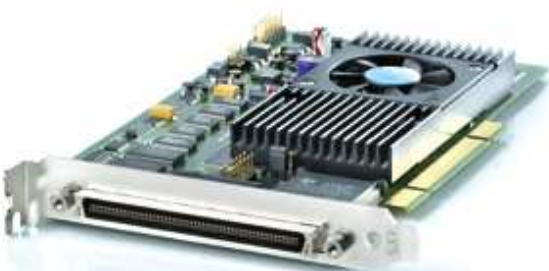
\includegraphics[width=0.4\textwidth]{Images/Ball and Bean/DS1104.png}
            \caption{Controller Board}
            \label{fig1}
        \end{figure}
    \item Dongle licenses on a USB flash disk
        \begin{figure}[H]
            \centering
            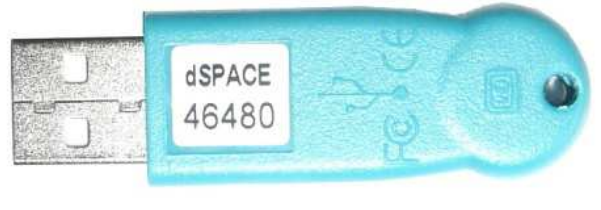
\includegraphics[width=0.25\textwidth]{Images/Ball and Bean/Dongle.png}
            \caption{Dongle USB flash}
            \label{fig2}
        \end{figure}
    \item Connector panel CLP1104
        \begin{figure}[H]
            \centering
            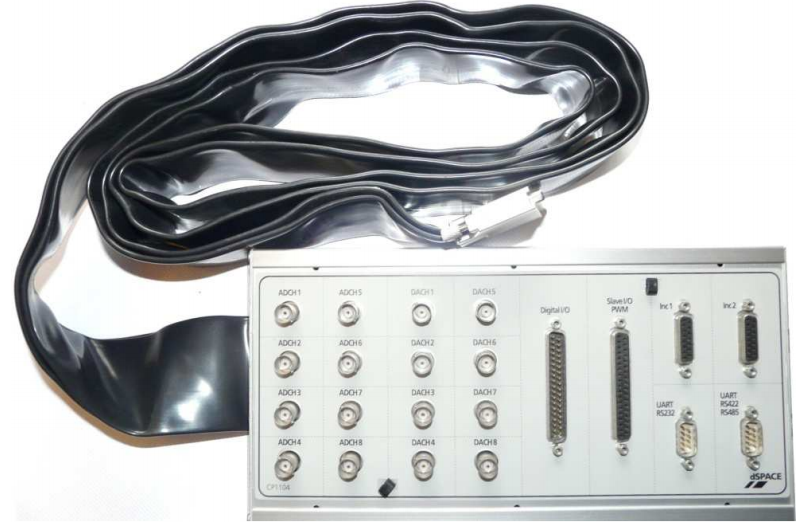
\includegraphics[width=0.5\textwidth]{Images/Ball and Bean/CLP1104.png}
            \caption{Connector panel}
            \label{fig3}
        \end{figure}
    \item D Sub 37 cable connector
        \begin{figure}[H]
            \centering
            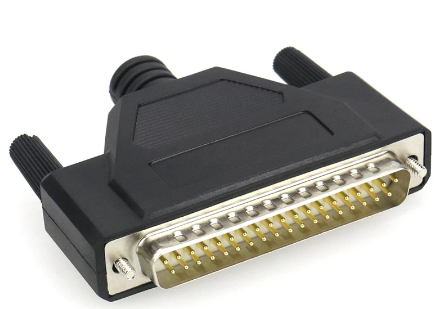
\includegraphics[width=0.35\textwidth]{Images/Ball and Bean/D-Sub37.png}
            \caption{Cable connector}
            \label{fig3.1}
        \end{figure}
    \item Servomotor Futaba S3003
        \begin{figure}[H]
            \centering
            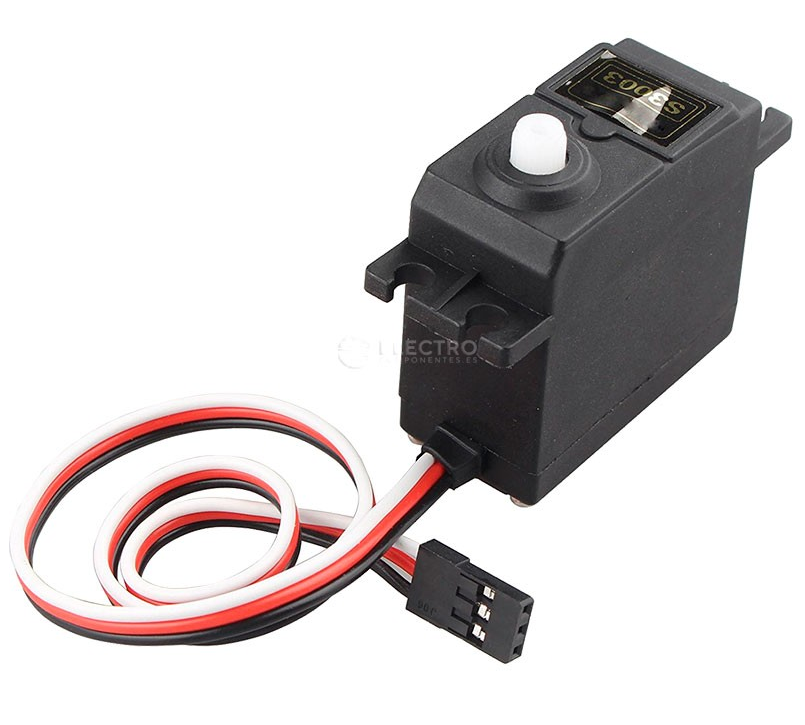
\includegraphics[width=0.4\textwidth]{Images/Ball and Bean/Servo.png}
            \caption{Futaba S3003}
            \label{fig3.2}
        \end{figure}
    \item Ultrasonic sensor HC-SR04
        \begin{figure}[H]
            \centering
            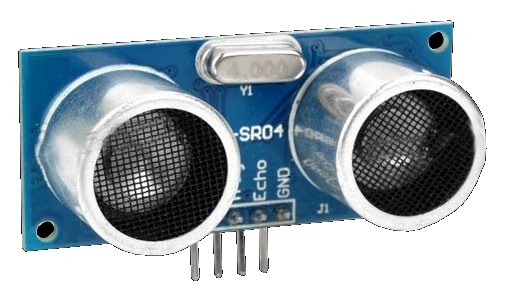
\includegraphics[width=0.4\textwidth]{Images/Ball and Bean/HC-SR04.png}
            \caption{HC-SR04}
            \label{fig3.3}
        \end{figure}
        
\end{enumerate}
\newpage

\section{Controller Design and Implementation in Simulink}
\subsection{Configuration of the Simulink model}
\begin{enumerate}
    
    \item The first step is start MATLAB and then, the following message appears, which says that dSPACE RealTime Interface (RTI) is installed for several hardware platforms, in this case, select DS1104.
    \begin{figure}[H]
        \centering
        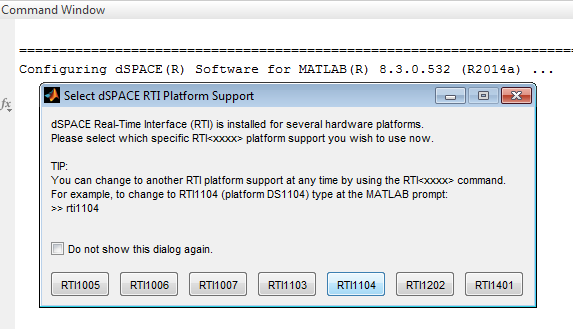
\includegraphics[width=0.7\textwidth]{Images/Ball and Bean/MatLab1.png}
        \caption{Selection of the RTI platform}
        \label{fig4}
    \end{figure}
By default, the workspace is placed in the user documents.
For a better organization of the generated files, change it to another directory because when you compile the Simulink model a \textbf{.sdf} file will be generated and without it, you won`t be able to work in the ControlDesk platform.
    
    
    \item  Some parameters must be adjusted before importing the model to ControlDesk. First, the solver and step time must be configured. To do so, click on the ‘Simulation’ button, and click on the option ‘Model Configuration Parameters’, which will open a new dialog window, as the one seen in figure \ref{fig6}. In ‘Solver Options’, select the type ‘Fixed-step’ and select the solver ‘ode4 (Runge-Kutta)’. In the option ‘Fixed-step size (fundamental sample time)’, a value must be entered such as it allows to have a good resolution of data capture, for this project, a value between 0.001 and 0.0001 is admissible.
    \begin{figure}[H]
        \centering
        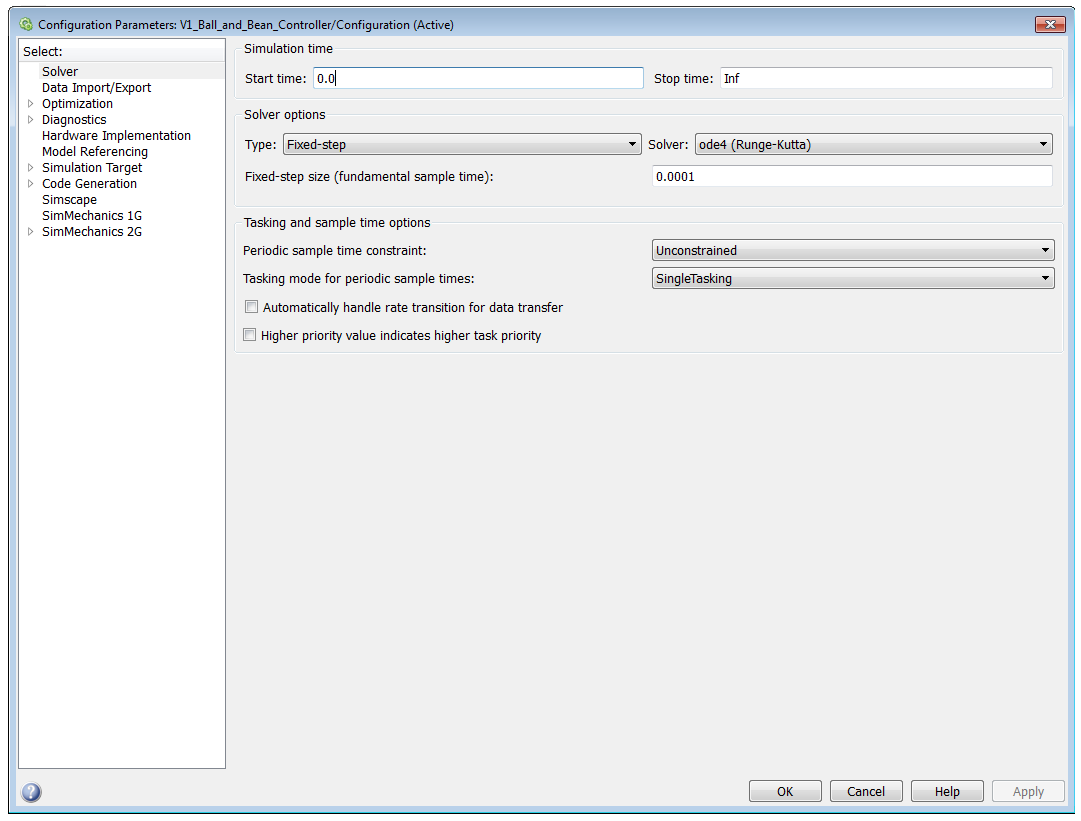
\includegraphics[width=0.7\textwidth]{Images/Ball and Bean/MatLab5.png}
        \caption{Configuration of integration step}
        \label{fig6}
    \end{figure}

    \item The option ‘Simulation Time’ must be set to ‘inf’. This can be done in the option ‘Solver’ of the ‘Model Configuration Parameters’ window, or in the box shown in the toolbar of Simulink, as seen in figure \ref{fig7}. This allows ControlDesk to simulate the model for an indefinite amount of time, instead of stopping the simulation at a specific time, as it is done normally in Simulink.
    \begin{figure}[H]
        \centering
        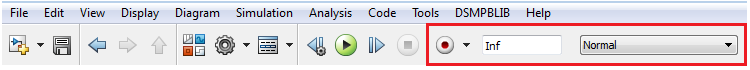
\includegraphics[width=0.7\textwidth]{Images/Ball and Bean/MatLab6.png}
        \caption{Change of simulation time to ‘Inf’}
        \label{fig7}
    \end{figure}

    \item The model must be saved as a .slx file in the main folder defined by the user in step 1.

    \item Finally, the model must be compiled in the dSPACE board. The DS1104 board must be selected in the ‘Model Configuration Parameters’ window, selecting the ‘Code Generation’ option, as seen in the figure \ref{fig8}. Press the button ‘Browse. . . ’ at the right of ‘System target file’ to open a window that will show a list of .tlc files, and select the one associated with the DS1104 board, as shown in figure \ref{fig9}.
    \begin{figure}[H]
        \centering
        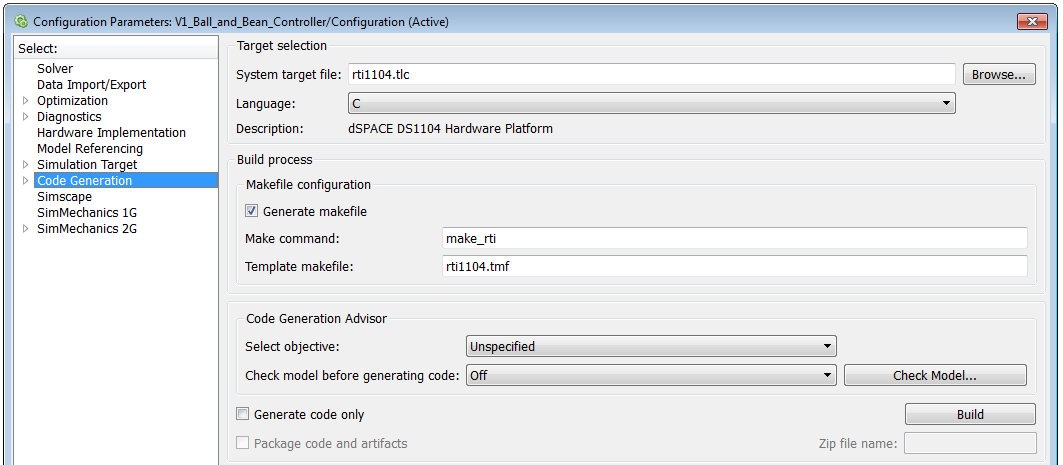
\includegraphics[width=0.7\textwidth]{Images/Ball and Bean/MatLab7.png}
        \caption{Selection of the board for compilation}
        \label{fig8}
    \end{figure}
    
    \begin{figure}[H]
        \centering
        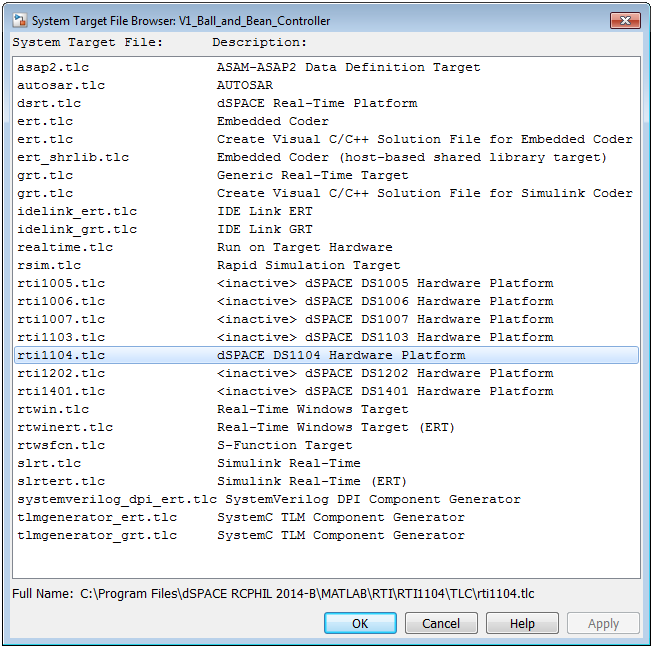
\includegraphics[width=0.7\textwidth]{Images/Ball and Bean/MatLab8.png}
        \caption{ Selection of the .tlc file related to the board}
        \label{fig9}
    \end{figure}

    \item The final step is to generate the code that will be compiled in the board. In Simulink, go to the menu ‘Code’, and in the option ‘C/C++ Code’ select ‘Build model’, as seen in figure \ref{fig10} or press \textbf{Ctrl+B}. If it is the first time this process is done after opening MATLAB, the error shown in figure \ref{fig11} will appear in the ‘Diagnostic Viewer’ window. To solve the issue, paste the code shown in the message \textbf{revertInlineParameterOffTo2013b} in the command window of MATLAB and press enter. The message shown in figure \ref{fig12} will appear. In the Simulink model, an icon will appear (‘RTI Data’), showing that the model is associated with a Real Time Interface, as seen in figure \ref{fig13}. A .sdf file, along with other files and folders will appear in the route selected in MATLAB.
    \begin{figure}[H]
        \centering
        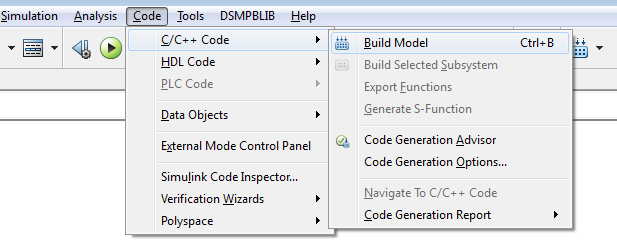
\includegraphics[width=0.7\textwidth]{Images/Ball and Bean/MatLab9.png}
        \caption{Generation of C code}
        \label{fig10}
    \end{figure}
    
    \begin{figure}[H]
        \centering
        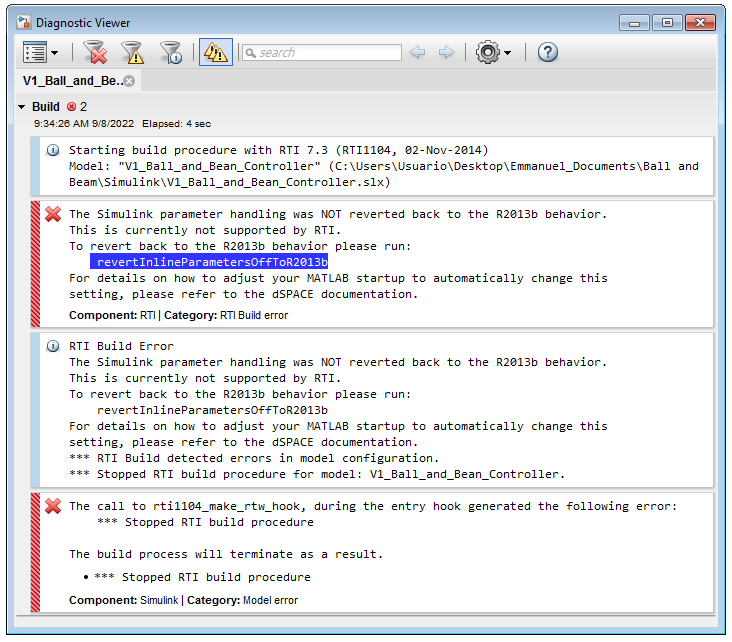
\includegraphics[width=0.7\textwidth]{Images/Ball and Bean/MatLab10.png}
        \caption{RTI Error message}
        \label{fig11}
    \end{figure}
    
    \begin{figure}[H]
        \centering
        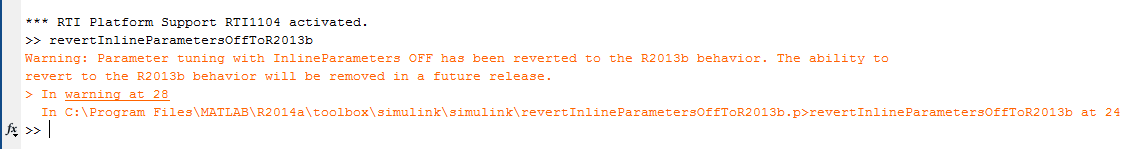
\includegraphics[width=0.7\textwidth]{Images/Ball and Bean/MatLab11.png}
        \caption{Command window of MATLAB after the correction of the error}
        \label{fig12}
    \end{figure}
    
    \begin{figure}[H]
        \centering
        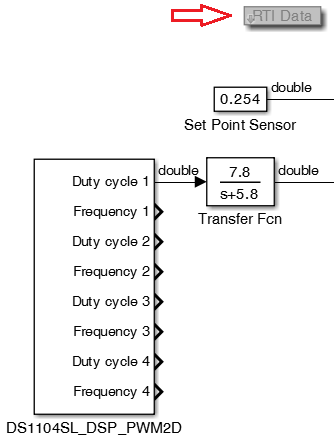
\includegraphics[width=0.5\textwidth]{Images/Ball and Bean/MatLab12.png}
        \caption{‘RTI Data’ symbol in the Simulink model}
        \label{fig13}
    \end{figure}
\end{enumerate}

\subsection{dSPACE Simulink blocks}

In Simulink, there is available a library of blocks related to the dSPACE board.
    
    \begin{figure}[H]
        \centering
        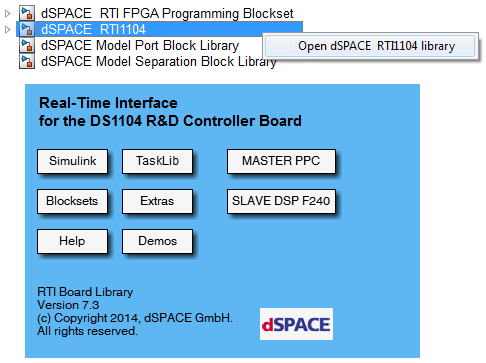
\includegraphics[width=0.7\textwidth]{Images/Ball and Bean/MatLab4.png}
        \caption{dSPACE libraries in Simulink.}
        \label{fig5}
    \end{figure}
By clicking on the SLAVE DSP F240 button, the window shown in figure \ref{fig14} be displayed.

     \begin{figure}[H]
        \centering
        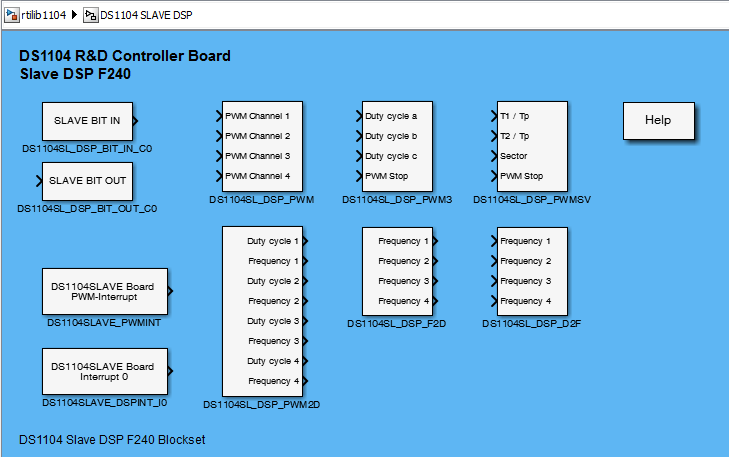
\includegraphics[width=0.7\textwidth]{Images/Ball and Bean/MatLab13.png}
        \caption{DS1104 Slave DSP F240 Blockset}
        \label{fig14}
    \end{figure}
Here you can find all the blocks related to the DS1104 slave DSP module.
For this project only two blocks will be needed:
\begin{enumerate}
    \item \textbf{DS1104SL\_DSP\_PWM}: for 1 phase PWM generation.
    \item \textbf{DS1104SL\_DSP\_PWM2D}: for sensor echo reading.
\end{enumerate}

\subsection{Basics of Slave DSP PWM Signal Generation}
The slave DSP of the DS1104 provides outputs for PWM signal generation. Each PWM pulse is centered around the middle of the corresponding PWM period (symmetric PWM generation mode) or in phase with the start of the period (asymmetric PWM generation mode).

\noindent \textbf{PWM signals}\par

PWM signal generation is crucial to many motor and motion control applications. PWM signals are pulse trains with fixed frequency and magnitude and variable pulse width. There is one pulse of fixed magnitude in every PWM period.

However, the width of the pulses changes from period to period according to a modulating signal. When a PWM signal is applied to the gate of a power transistor, it causes the turn-on/turn-off intervals of the transistor to change from one PWM period to another, according to the same modulating signal. The frequency of a PWM signal is usually much higher than that of the modulating signal, or the fundamental frequency, so that the energy delivered to the motor and its load depends mainly on the modulating signal.

\noindent \textbf{PWM period, duty cycle and resolution}\par

For PWM signals, you can specify the PWM period TP (= T$_high$+ T$_low$) in the range 200 ns … 819,2 ms. For 1-phase PWM signals, the PWM period TP applies to each of the four PWM output channels.

You can also specify the duty cycle. The following illustration shows how the duty cycle d (= T$_high$/ TP) is defined. The available duty cycle range is 0 … 1 (0 … 100 \%).

\begin{figure}[H]
    \centering
    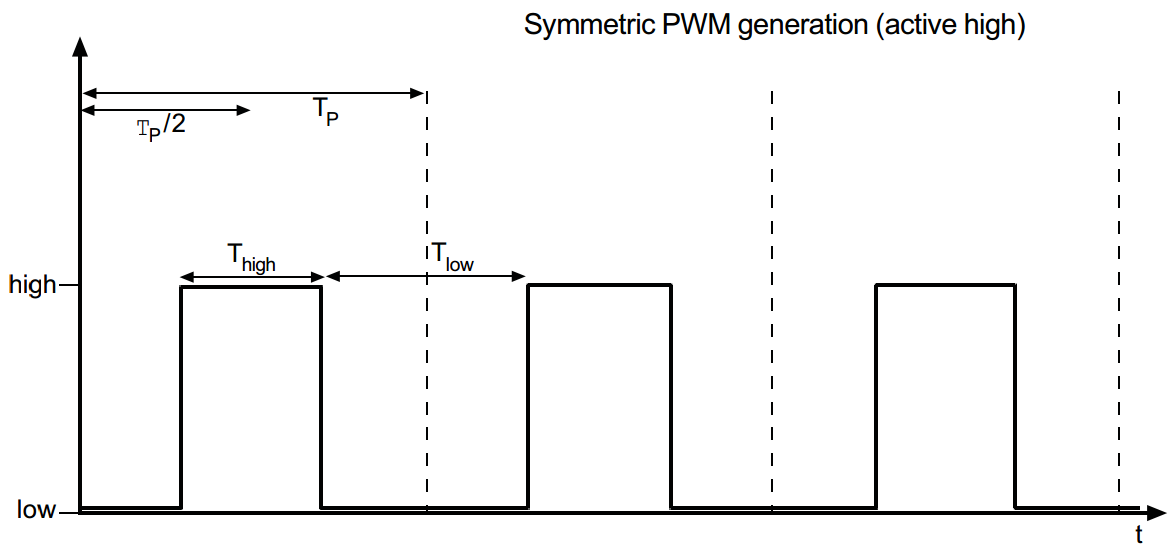
\includegraphics[width=\textwidth]{Images/Symmetric PWM generation.png}
    \caption{Symmetric PWM generation}
    %\label{Symmetric PWM generation}
\end{figure}

Depending on the selected PWM period, the following resolutions are given. They apply to symmetric PWM signals.

\begin{table}[H]
\centering
\begin{tabular}{|l|l|}
\hline
\rowcolor[HTML]{34CDF9} 
\textbf{Period T$_p$} & \textbf{Resolution} \\ \hline
\textless 6.4 ms   & 100 ns              \\
\textless 12.8 ms  & 200 ns              \\
\textless 25.6 ms  & 400 ns              \\
\textless 51.2 ms  & 800 ns              \\
\textless 102.4 ms & 1.6 $\mu$s              \\
\textless 204.8 ms & 3.2 $\mu$s              \\
\textless 409.6 ms & 6.4 $\mu$s              \\
\textless 819.2 ms & 12.8 $\mu$s             \\ \hline
\end{tabular}
\caption{Symmetric PWM resolution}
%\label{Symmetric PWM resolution}
\end{table}

\noindent \textbf{Asymmetric PWM mode}

As an alternative to the symmetric PWM generation mode, you can also let each PWM pulse start at the beginning of the corresponding PWM period (asymmetric PWM mode). Switching between symmetric and asymmetric PWM mode applies to all of the four 1-phase PWM output channels. The following illustration shows two active high symmetric and asymmetric 1-phase PWM signals.
\begin{figure}[H]
    \centering
    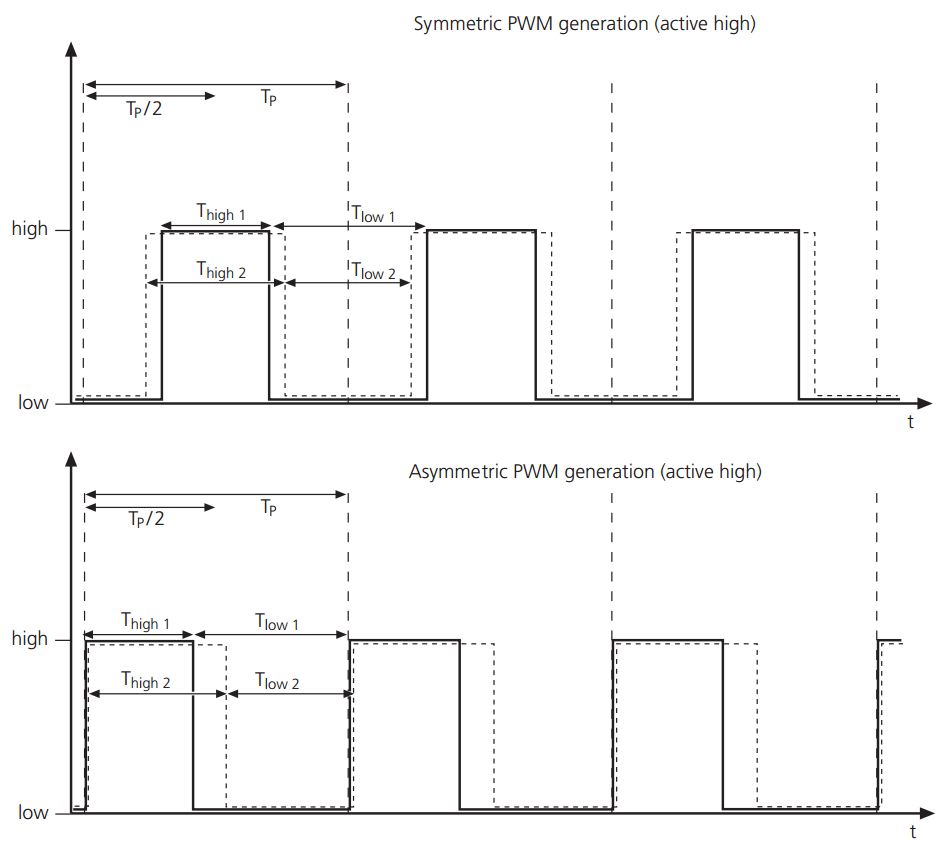
\includegraphics[width=0.8\textwidth]{Images/Symmetric and asymmetric PWM generation.png}
    \caption{Symmetric and asymmetric PWM generation}
    %\label{Symmetric and asymmetric PWM generation}
\end{figure}

\noindent \textbf{PWM period and resolution in asymmetric mode}\par

In the asymmetric mode, the PWM period T$_P$ must be in the range 200 ns … 409,6 ms. Depending on the period, the following resolutions are given:

\begin{table}[H]
\centering
\begin{tabular}{|l|l|}
\hline
\rowcolor[HTML]{34CDF9} 
\textbf{Period T$_p$} & \textbf{Resolution} \\ \hline
\textless 3.2 ms   & 50 ns              \\
\textless 6.4 ms   & 100 ns              \\
\textless 12.8 ms  & 200 ns              \\
\textless 25.6 ms  & 400 ns              \\
\textless 51.2 ms  & 800 ns              \\
\textless 102.4 ms & 1.6 $\mu$s              \\
\textless 204.8 ms & 3.2 $\mu$s              \\
\textless 409.6 ms & 6.4 $\mu$s              \\ \hline
\end{tabular}
\caption{Asymmetric PWM resolution}
%\label{Asymmetric PWM resolution}
\end{table}
\noindent \textit{Due to quantization effects, you will encounter considerable deviations between the desired PWM period T$_P$ and the generated PWM period, especially for higher PWM frequencies.}

\noindent \textbf{PWM outputs}\par
The PWM outputs can be specified. The running PWM generation can be suspended and the corresponding channels can be set to a specified TTL level (high or low). Only the output of the PWM signal is disabled. Signal calculation is still running and if you enable PWM generation, the currently calculated signal is output, and not the defined initialization or termination value. The PWM outputs can be specified for the two simulation phases (RTI):
\begin{itemize}
    \item During the initialization phase, you can disable the PWM generation of selected channels and set each output (pair) to a defined TTL level (high or low). No signal is generated during the initialization.
    \item During run time, you can stop PWM generation and set the outputs to a defined TTL level (high or low). At any time you can resume in generating the PWM signal. If the simulation terminates the outputs can be set to defined TTL levels.
\end{itemize}

If the PWM stop feature is disabled, the normal initialization and termination routines are executed. That means the specified duty cycles for initialization and termination are used.

\subsection{1-Phase PWM Signal Generation - DS1104SL\_DSP\_PWM}

    \begin{figure}[H]
        \centering
        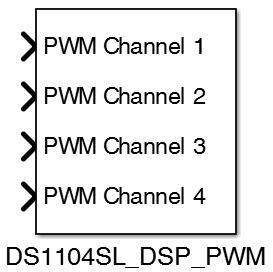
\includegraphics[width=0.35\textwidth]{Images/Ball and Bean/MatLab14.png}
        \caption{DS1104SL\_DSP\_PWM module in Simulink}
        \label{fig15}
    \end{figure}

\noindent \textbf{Purpose}\par
To generate standard PWM signals with variable duty cycles and enable PWM stop during run time.

\noindent \textbf{Description}\par 
For 1-phase PWM generation, a PWM stop can be specified to suspend PWM signal output during run time. The outputs of the channels are set to a defined TTL level. The dimensions of the inports are set to 2, which allows you to enter two values over the same port. This can be done via a Simulink MUX block, for example. Value 1 specifies the duty cycle and value 2 the PWM stop behavior. If you set value 2 to “0” a PWM signal is generated, “1” suspends signal generation and sets the output to the specified TTL level. If the PWM stop is disabled for a channel only the duty cycle can be input. Although you can disable the PWM stop feature for each channel during run time, you can specify whether you want to set the PWM output to a specified TTL level or to generate a signal during the initialation phase.

\noindent \textbf{I/O mapping}\par 

\begin{table}[H]
\begin{adjustbox}{width=1\textwidth}
\small
\begin{tabular}{|lllll|}
\hline
\rowcolor[HTML]{34CDF9} 
\multicolumn{1}{|l|}{\cellcolor[HTML]{34CDF9}\textbf{Signal}} &
  \multicolumn{3}{l|}{\cellcolor[HTML]{34CDF9}\textbf{Channel/Bit Numbers of Related RTI Blocks/RTLib Functions}} &
  {\cellcolor[HTML]{34CDF9}\textbf{I/O Pin on …}} \\ \cline{2-5} 
\rowcolor[HTML]{34CDF9} 
\multicolumn{1}{|l|}{\cellcolor[HTML]{34CDF9}\textbf{}} &
  \multicolumn{1}{l|}{\cellcolor[HTML]{34CDF9}\textbf{Related RTI Block(s)}} &
  \multicolumn{1}{l|}{\cellcolor[HTML]{34CDF9}\textbf{Ch/Bit (RTI)}} &
  \multicolumn{1}{l|}{\cellcolor[HTML]{34CDF9}\textbf{Ch/Bit (RTILib)}} &
  \textbf{D-SUB 37} \\ \hline
\multicolumn{5}{|l|}{\textbf{1‑Phase PWM Signal Generation (PWM)}} \\ \hline
\multicolumn{5}{|l|}{\tabitem TTL output voltage range} \\
\multicolumn{5}{|l|}{\tabitem Output current range: ±13 mA} \\
\multicolumn{1}{|l|}{ST2PWM} &
  \multicolumn{1}{l|}{DS1104SL\_DSP\_PWM} &
  \multicolumn{1}{l|}{Channel 1} &
  \multicolumn{1}{l|}{Channel 1} &
  5 \\
\multicolumn{1}{|l|}{SPWM7} &
  \multicolumn{1}{l|}{} &
  \multicolumn{1}{l|}{Channel 2} &
  \multicolumn{1}{l|}{Channel 2} &
  10 \\
\multicolumn{1}{|l|}{SPWM8} &
  \multicolumn{1}{l|}{} &
  \multicolumn{1}{l|}{Channel 3} &
  \multicolumn{1}{l|}{Channel 3} &
  29 \\
\multicolumn{1}{|l|}{SPWM9} &
  \multicolumn{1}{l|}{} &
  \multicolumn{1}{l|}{Channel 4} &
  \multicolumn{1}{l|}{Channel 4} &
  11 \\ \hline
\end{tabular}
\end{adjustbox}
\caption{Slave DSP 1-phase PWM Signal}
\label{Slave DSP 1-phase PWM Signal}
\end{table}

\noindent \textbf{I/O characteristics}\par

\begin{table}[H]
\begin{adjustbox}{width=1\textwidth}
\begin{tabular}{|l|l|l|l|l|}
\hline
\rowcolor[HTML]{34CDF9} 
\textbf{Simulink Inport} & \textbf{Input}   & \textbf{Value} & \textbf{Data Type} & \textbf{Meaning}                                 \\ \hline
PWM Channel 1 … 4        & Duty cycle 1 … 4 & 0 ... 1        & Double             & Duty cycle of the PWM signal for channel 1 ... 4 \\
                         & PWM Stop 1 … 4   & 0 ... 1        & Boolean            & Enables PWM stop for channel 1 … 4:              \\
 &  &  &  & \tabitem Value 1 stops PWM generation   \\
 &  &  &  & \tabitem Value 0 resumes PWM generation \\ \hline
\end{tabular}
\end{adjustbox}
\caption{1-phase PWM Signal Simulink data types}
\label{1-phase PWM Signal Simulink data types}
\end{table}

\subsubsection{Simulink implementation}
The DS1104SL\_DSP\_PWM inputs PWM Channel 1 ... 3 were used and channel 4 was disabled.
\begin{itemize}
    \item \textbf{PWM Channel 1}, is used for pulse generation for triggering the HC-SR04 ultrasonic sensor.
    \item \textbf{PWM Channel 2}, is used to command the servo motor linked to the sensor and the ball guide.
    \item \textbf{PWM channel 3}, is used to lock the two servo motors of the base. Just to make sure that nothing will move unintentionally.
    \item \textbf{PWM channel 4}, disabled.
\end{itemize}
The block was configured to operate at \textcolor{red}{\textbf{50 Hz}} in \textcolor{red}{\textbf{asymmetric mode}}. All other parameters were left at their default values.
Like mentioned above, all four inputs were multiplexed with a \textcolor{red}{\textbf{STOP bit}} to provide the start/stop option.
    \begin{figure}[H]
        \centering
        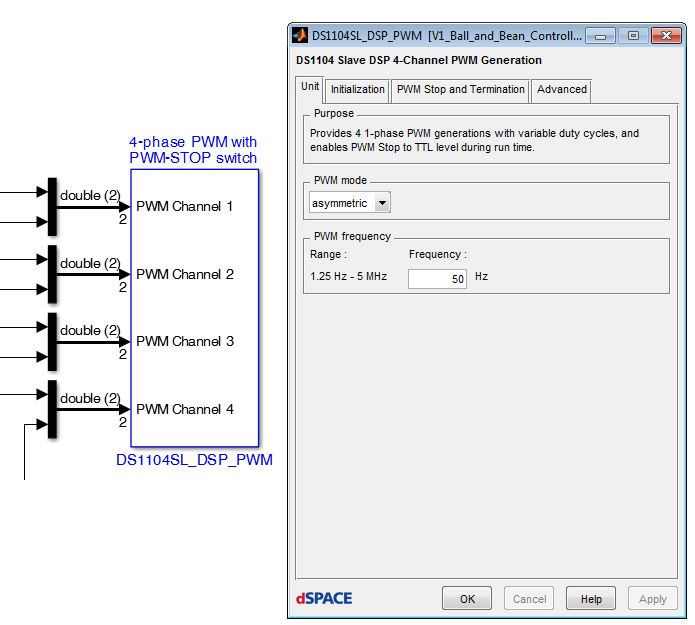
\includegraphics[width=0.7\textwidth]{Images/Ball and Bean/MatLab17.png}
        \caption{PWM module in Simulink}
        \label{fig18}
    \end{figure}

\subsection{1-Phase PWM Signal Measurement - DS1104SL\_DSP\_PWM2D}
In this case the DS1104SL\_DSP\_PWM2D block is used.\par
It can measure the duty cycles and the frequencies from up to 4 independent channels used for PWM-type signals.\\
The reason for its use is because the HC-SR04 returns a high pulse proportional to the duration of the echo of the sound emitted by the sensor actuator.\par
The measurement algorithm used is accurate if the PWM period starts
with the falling or rising edge of the corresponding PWM signal so, the PWM module must be in \textcolor{red}{\textbf{asymmetric mode}}.\par
As only one signal will be measured, channel 1 is used to measure its duty cycle.

\begin{table}[H]
\begin{adjustbox}{width=1\textwidth}
\small
\begin{tabular}{|lllll|}
\hline
\rowcolor[HTML]{34CDF9} 
\multicolumn{1}{|l|}{\cellcolor[HTML]{34CDF9}\textbf{Signal}} &
  \multicolumn{3}{l|}{\cellcolor[HTML]{34CDF9}\textbf{Channel/Bit Numbers of Related RTI Blocks/RTLib Functions}} &
  {\cellcolor[HTML]{34CDF9}\textbf{I/O Pin on …}} \\ \cline{2-5} 
\rowcolor[HTML]{34CDF9} 
\multicolumn{1}{|l|}{\cellcolor[HTML]{34CDF9}\textbf{}} &
  \multicolumn{1}{l|}{\cellcolor[HTML]{34CDF9}\textbf{Related RTI Block(s)}} &
  \multicolumn{1}{l|}{\cellcolor[HTML]{34CDF9}\textbf{Ch/Bit (RTI)}} &
  \multicolumn{1}{l|}{\cellcolor[HTML]{34CDF9}\textbf{Ch/Bit (RTILib)}} &
  \textbf{D-SUB 37} \\ \hline
\multicolumn{5}{|l|}{\textbf{Slave DSP PWM Signal Measurement (PWM2D)}} \\ \hline
\multicolumn{5}{|l|}{\tabitem TTL input voltage range 0 - 5V} \\
\multicolumn{5}{|l|}{\tabitem Input current: 500 $\mu$A} \\
\multicolumn{1}{|l|}{SCAP1} &
  \multicolumn{1}{l|}{DS1104SL\_DSP\_PWM2D} &
  \multicolumn{1}{l|}{Channel 1} &
  \multicolumn{1}{l|}{Channel 1} &
  2 \\
\multicolumn{1}{|l|}{SCAP2} &
  \multicolumn{1}{l|}{} &
  \multicolumn{1}{l|}{Channel 2} &
  \multicolumn{1}{l|}{Channel 2} &
  21 \\
\multicolumn{1}{|l|}{SCAP3} &
  \multicolumn{1}{l|}{} &
  \multicolumn{1}{l|}{Channel 3} &
  \multicolumn{1}{l|}{Channel 3} &
  3 \\
\multicolumn{1}{|l|}{SCAP4} &
  \multicolumn{1}{l|}{} &
  \multicolumn{1}{l|}{Channel 4} &
  \multicolumn{1}{l|}{Channel 4} &
  22 \\ \hline
\end{tabular}
\end{adjustbox}
\caption{Signal mapping of Slave DSP PWM Signal Measurement (PWM2D)}
\label{Signal mapping of Slave DSP PWM Signal Measurement (PWM2D)}
\end{table}
    \begin{figure}[H]
        \centering
        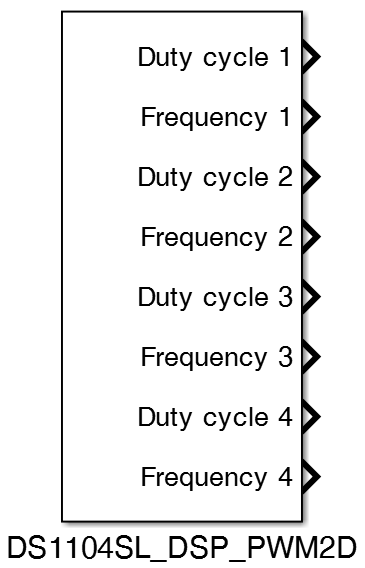
\includegraphics[width=0.4\textwidth]{Images/Ball and Bean/MatLab15.png}
        \caption{Measurement module in Simulink}
        \label{fig19}
    \end{figure}

\newpage

\subsection{Basic Operation and Timing of the HC-SRO4 Ultrasonic Sensor}

    \begin{figure}[H]
        \centering
        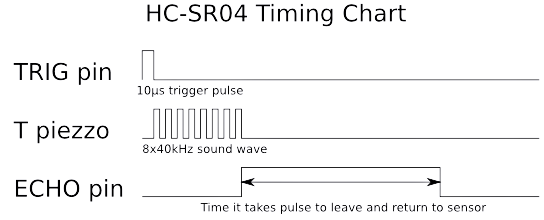
\includegraphics[width=0.6\textwidth]{Images/Ball and Bean/HC-SR04-Timing.png}
        \caption{HC-SR04 Timing chart}
        \label{fig20}
    \end{figure}
    \begin{enumerate}
        \item Make "Trig" (pin 2) on the sensor high for 10µs. This initiates a sensor cycle.
        \item 8x40kHz pulses will be sent from the "T" transmitting piezzo transducer of the sensor, after which time the "Echo" pin on the sensor will go from low to high.
        \item The 40kHz sound wave will bounce off the nearest object and return to the sensor.
        \item When the sensor detects the reflected sound wave, the the Echo pin will go low again.
        \item The distance between the sensor and the detected object can be calculated based on the length of time the Echo pin is high.
        \item If no object is detected, the Echo pin will stay high for 38ms and then go low.
    \end{enumerate}
    
\subsection{Basic Operation and Timing of Futaba S3003 Servomotor}
    \begin{figure}[H]
        \centering
        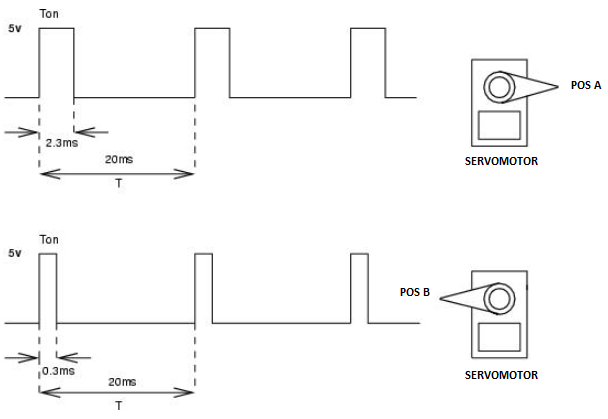
\includegraphics[width=0.5\textwidth]{Images/Ball and Bean/Servo2.png}
        \caption{Servomotor Timing chart}
        \label{fig21}
    \end{figure}
To position the servo, a periodic signal of 50Hz (20ms period) must be applied. The width of the pulse determines the servo position. If the width is 2.3ms, the servo is positioned at one end and if the width is 0.3ms it is positioned at the opposite end. Any other width between 0.3 and 2.3ms places the servo in a position between one end and the other. For example, if we want it to be positioned exactly in the center, we apply a width of 1.3ms.

When the signal is no longer sent, the servo enters an idle state, and can therefore be moved by hand. As long as the signal is applied, it will remain fixed in its position, forcing it to stay there.

\subsection{Finding the limits of the servomotor - Simulink example model}

Simulink has the simplicity of block programming and the programmer must have the skills to realize a simple, efficient and robust control system.

You must know how your servo motor operate and especially its limits. You can build a simple model in Simulink and find these limits with ControlDesk. Not all motors are the same and to be accurate, this is a necessary step.

For this example a \textit{20ms} period will be set, that is the typical value for this type of servomotors (this value also change whit the servomotor model).
    \begin{figure}[H]
        \centering
        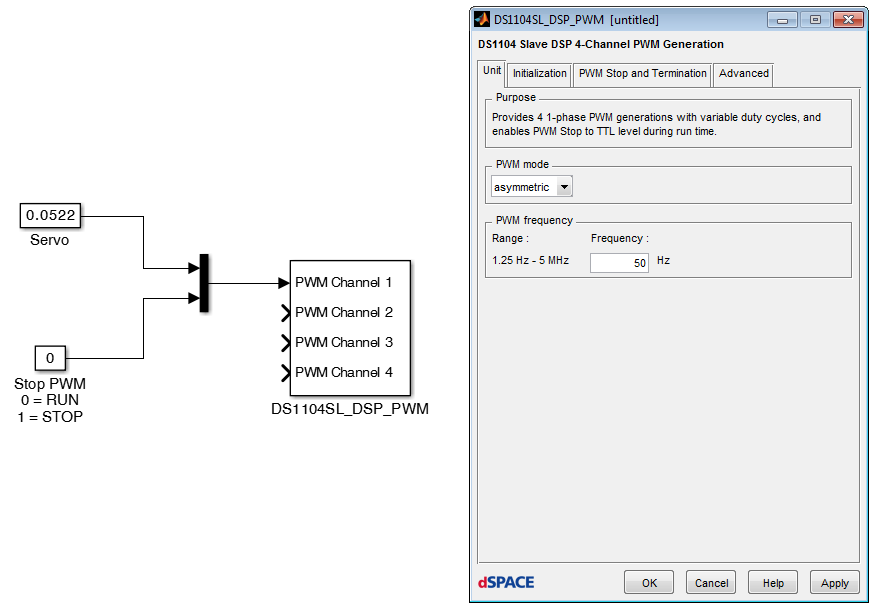
\includegraphics[width=0.6\textwidth]{Images/Ball and Bean/PWM_Example.png}
        \caption{Simulink servomotor test}
        \label{fig22}
    \end{figure}
You must now follow the compilation steps mentioned in the first section in order to work with ControDesk. After compilation process, the RTI Data symbol will appear.
       
     \begin{figure}[H]
        \centering
        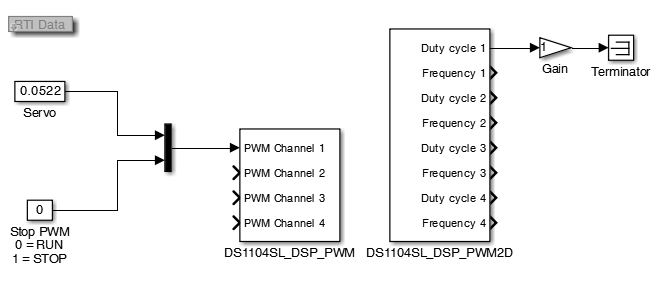
\includegraphics[width=0.8\textwidth]{Images/Ball and Bean/PWMExampleSimulink.png}
        \caption{Simulink model - servomotor test}
        \label{fig37}
    \end{figure}
    
With this model you will be able to test your servomotors to know their characteristics and operating limits.\par
Remember that most servomotors operate between 0,3 and 2,3 ms pulse width for their entire range of motion.
You can make a test using an oscilloscope to measure the pulse width.
Changing the \textcolor{green}{\textit{Servo input value}} in the ControlDesk interface you will notice than the pulse get bigger or smaller.
The following pictures show this example:
    \begin{figure}[H]
        \centering
        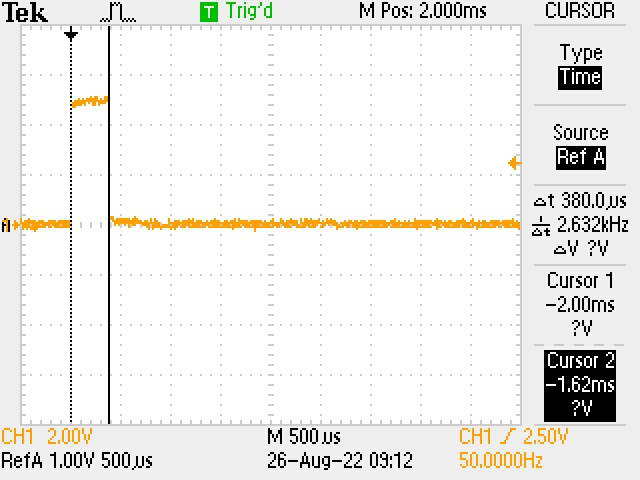
\includegraphics[width=0.5\textwidth]{Images/Servo_Pulse_Time/0.png}
        \caption{Pulse width at 0º angle - 380 $\mu$s}
        \label{fig38}
    \end{figure}
    \begin{figure}[H]
        \centering
        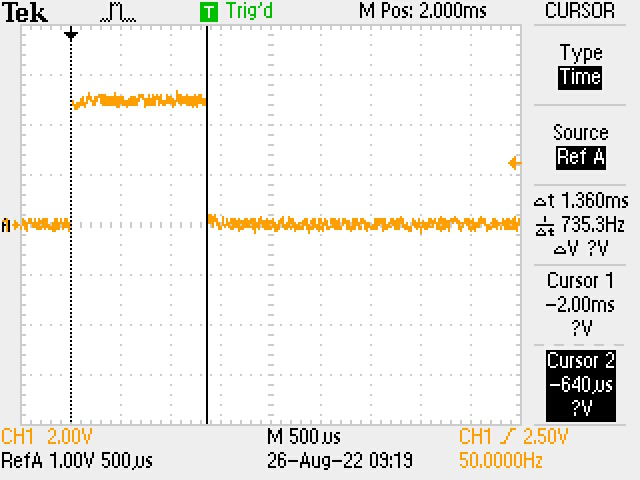
\includegraphics[width=0.5\textwidth]{Images/Servo_Pulse_Time/60.png}
        \caption{Pulse width at 60º angle - 1,36 ms}
        \label{fig39}
    \end{figure}
    \begin{figure}[H]
        \centering
        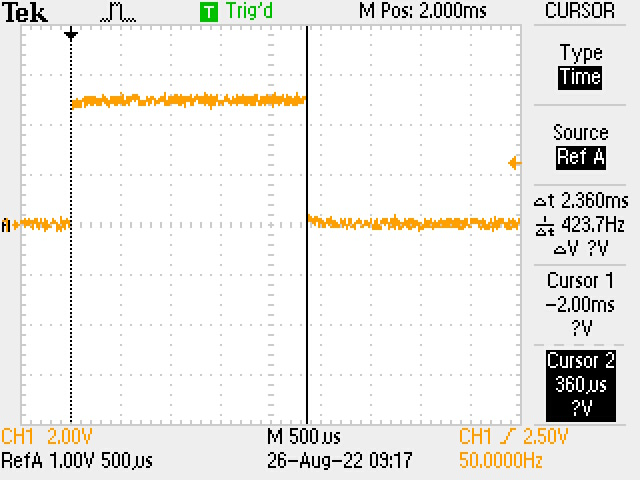
\includegraphics[width=0.5\textwidth]{Images/Servo_Pulse_Time/120.png}
        \caption{Pulse width at 120º angle - 2,36 ms}
        \label{fig40}
    \end{figure}

\subsection{ControlDesk interface}

\subsubsection{Creating a ControDesk project}
\begin{enumerate}
    \item Open ControlDesk 5.3. The first thing to do is to create a new project. This is done in the ‘File’ tab, in the option ‘New’, and selecting ‘Create New Project and Experiment’, as seen in figure \ref{fig24}.
    \begin{figure}[H]
        \centering
        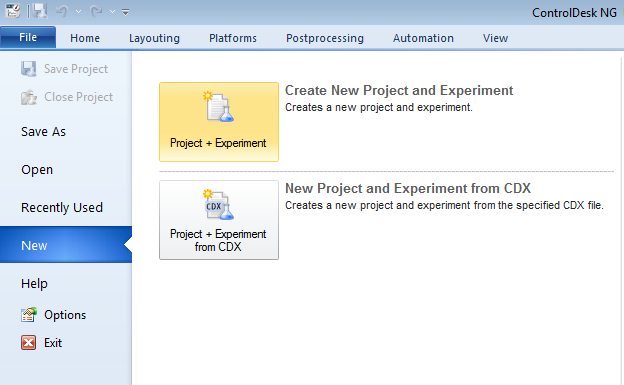
\includegraphics[width=0.5\textwidth]{Images/Ball and Bean/ControlDesk/CD1.png}
        \caption{Creation of a new project in ControlDesk}
        \label{fig24}
    \end{figure}
    \item A window will open. Select a name for the project and a root directory.
    \begin{figure}[H]
        \centering
        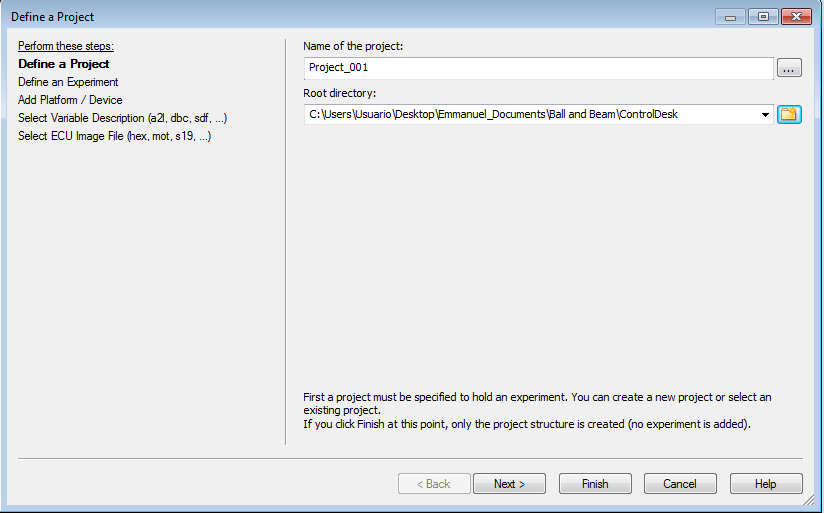
\includegraphics[width=0.5\textwidth]{Images/Ball and Bean/ControlDesk/CD2.png}
        \caption{Define a project}
        \label{fig25}
    \end{figure}
    \item The root directory must be in you project main folder. Just follow the steps in figure \ref{fig26}. 
    \begin{figure}[H]
        \centering
        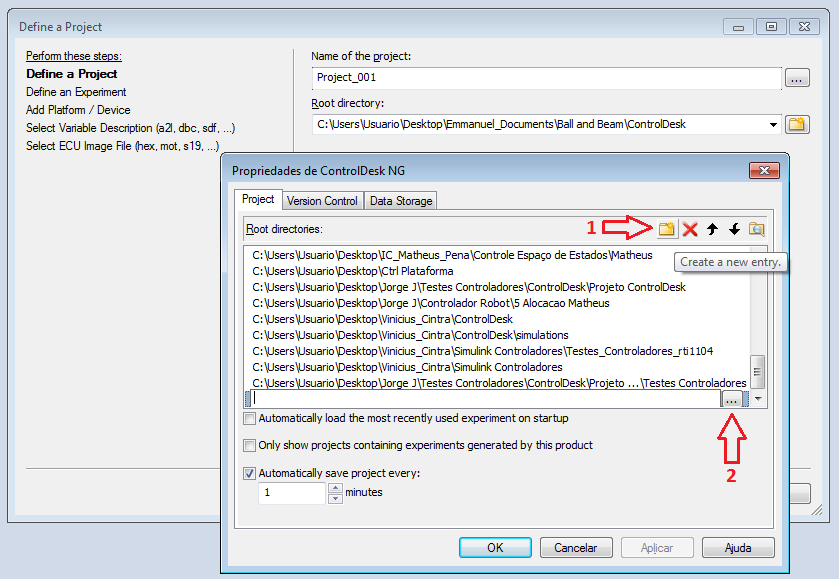
\includegraphics[width=0.5\textwidth]{Images/Ball and Bean/ControlDesk/CD3.png}
        \caption{Root directory}
        \label{fig26}
    \end{figure}
    \item After pressing ‘Next’, the user must select the controller board which is being used which, in this case, is the DS1104, as seen in figure \ref{fig27}.
    \begin{figure}[H]
        \centering
        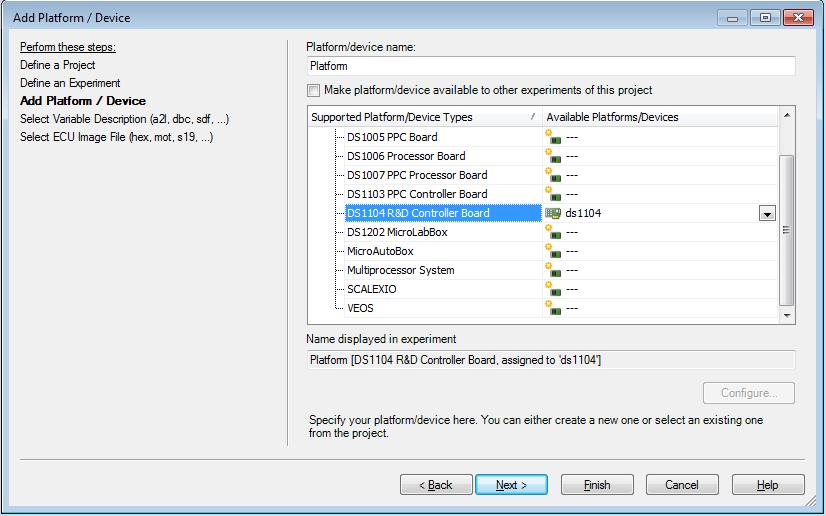
\includegraphics[width=0.5\textwidth]{Images/Ball and Bean/ControlDesk/CD4.png}
        \caption{Add plataform / Device}
        \label{fig27}
    \end{figure}
    \item To associate the variables from the Simulink model with ControlDesk, the \textcolor{red}{\textbf{.sdf}} file generated during the compilation of the code done previously must be imported by pressing the button ‘Import from file...’, and selecting it, as seen in figure \ref{fig28}. After this is done, press ‘Finish’.
    \begin{figure}[H]
        \centering
        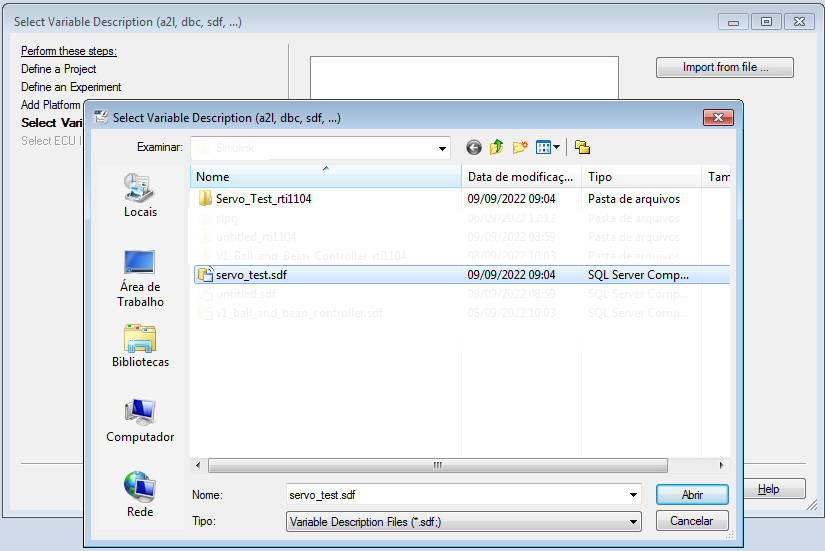
\includegraphics[width=0.5\textwidth]{Images/Ball and Bean/ControlDesk/CD5.png}
        \caption{Select variable description}
        \label{fig28}
    \end{figure}
    \item The software offers a variety of tools and options. The ones of interest are highlighted with colors in figure \ref{fig29}, are described below:
    \begin{itemize}
        \item Yellow area: corresponds to the lead toolbar.
        \item Red area: corresponds to the work area. In this zone, a variety of instruments like indicators, graphs, and numeric inputs can be placed, to create a ‘Layout’, which acts as a interface between the user and the controller.
        \item Blue area: the instrument selector shows all the instruments available. If this list does not appear at the moment the project is created, it can be activated in the menu ‘Layouting’, and selecting ‘Insert Instrument’.
        \item Green area: shows the variables associated with the imported Simulink model, or models. The instruments in the layout can be associated to variables of the Simulink model.
    \end{itemize}
    \begin{figure}[H]
        \centering
        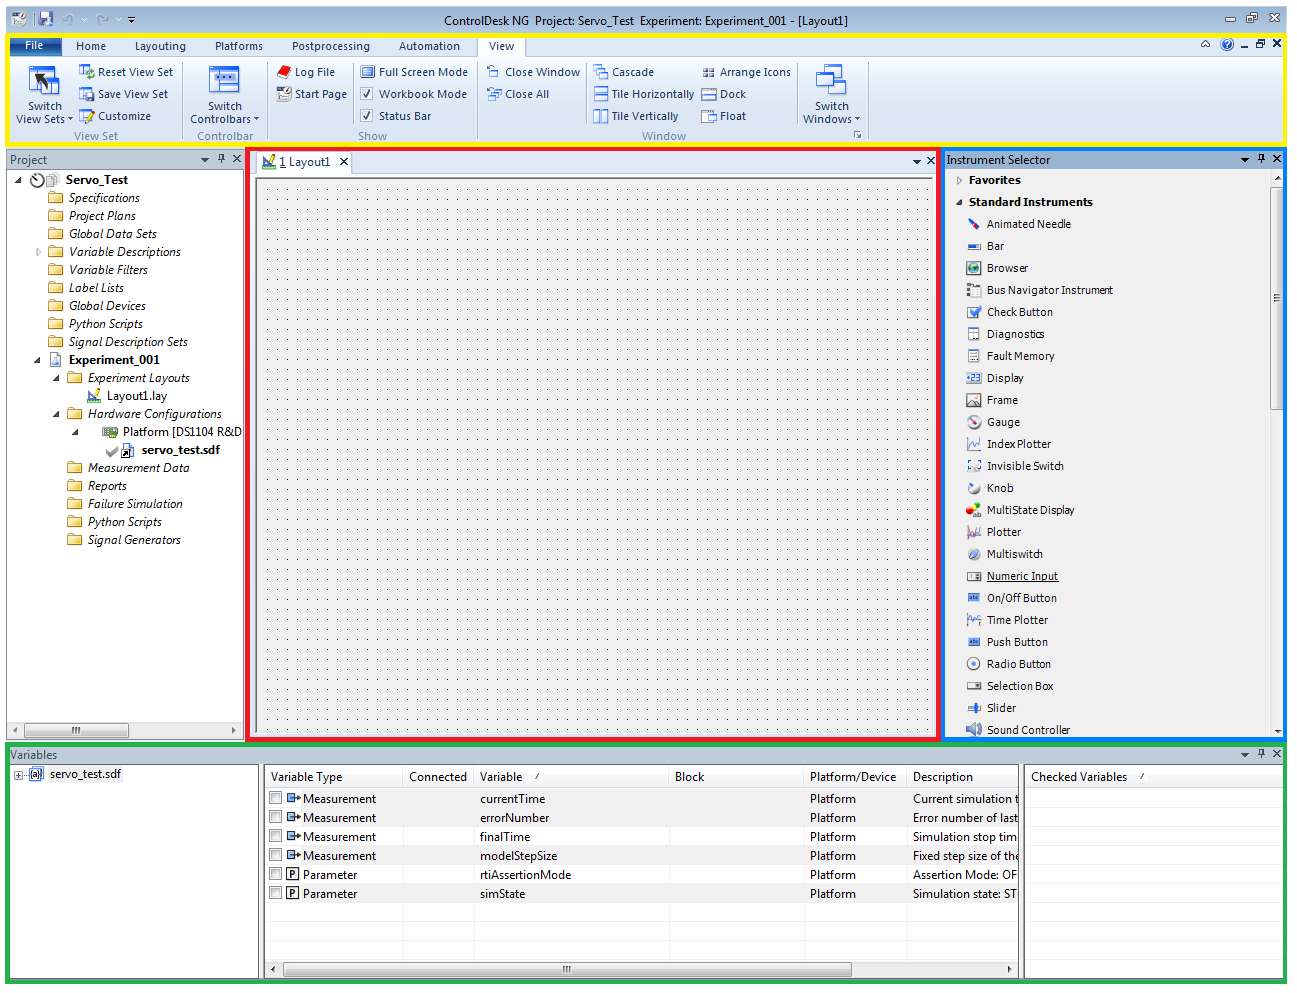
\includegraphics[width=0.8\textwidth]{Images/Ball and Bean/ControlDesk/CD6.png}
        \caption{ControlDesk window}
        \label{fig29}
    \end{figure}
    
\end{enumerate}


\subsubsection{Data recording}

\begin{enumerate}
    \item To be able to work with historical data of the variables, it is necessary to record their behavior during a real time experiment, and export them to a file. To analyze the data in MATLAB, a file can be generated with the recorder tool of ControlDesk. To display the ‘Measurement Configuration’ bar, go to the tab ‘View’, click on ‘Switch Controlbars’ and select ‘Measurement Configuration’, as seen in figure \ref{fig30}
    \begin{figure}[H]
        \centering
        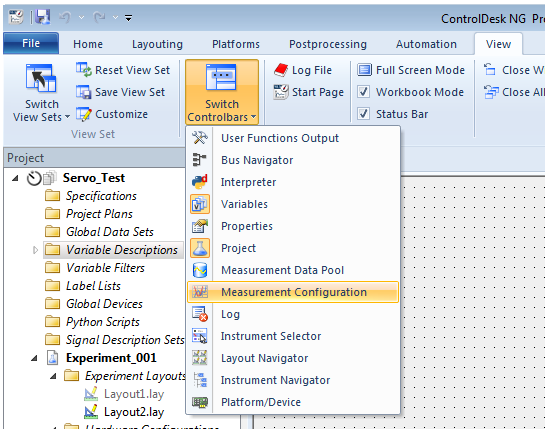
\includegraphics[width=0.8\textwidth]{Images/Ball and Bean/ControlDesk/CD7.png}
        \caption{Activation of the recording tool bar}
        \label{fig30}
    \end{figure}
    \item In the ‘Measurement Configuration’ bar one can find the ‘Recorders’. ControlDesk records the variables shown in the ‘Plotters’ of the layout by default, so the ‘Recorder 1’ corresponds to the actives plotters. To record another variable, one can drag and drop a variable from the ‘Variables’ bar to a existing recorder, or create one by right-clicking on ‘Recorders’, and selecting ‘Create New Recorder’.

    \item Right-click on ‘Recorder 1’ and select ‘Properties’ to open the dialog seen in figure \ref{fig31}. Select ‘Automatic export’ to automatically create a file with the recording of the variable, and select a name for the file, the folder where the file will be generated, and the file type. To be able to work the data in MATLAB select ‘MATLAB file (*.mat)’. Also, the name of the recorder can be changed
    \begin{figure}[H]
        \centering
        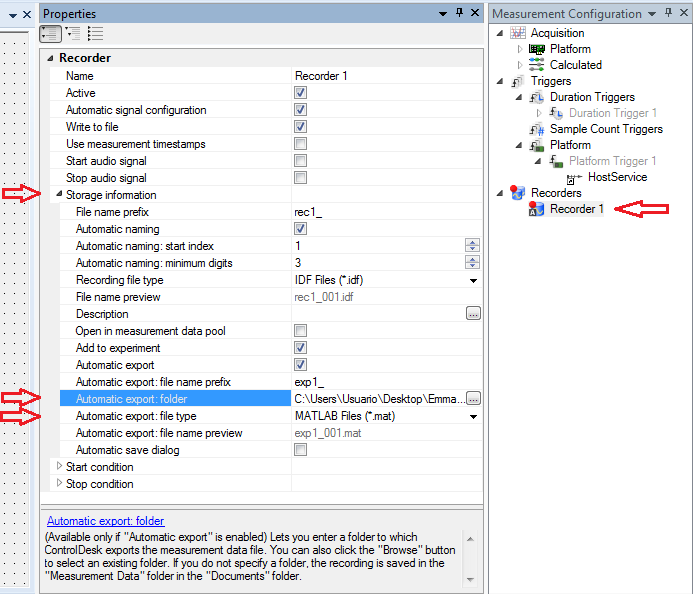
\includegraphics[width=0.8\textwidth]{Images/Ball and Bean/ControlDesk/CD8.png}
        \caption{Properties of the recorder}
        \label{fig31}
    \end{figure}

    \item To record the data, in the ‘Home’ tab, select ‘Start Immediate’ when the experiment is running, or any other time to initiate the experiment and record from the beginning. Also, the recording can be set to start automatically in response to a variable value or a logical expression, by selecting ‘Trigger Rules’.
    \begin{figure}[H]
        \centering
        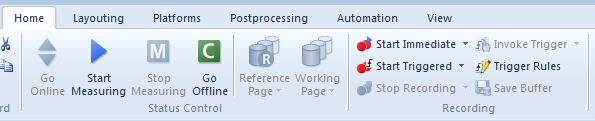
\includegraphics[width=0.8\textwidth]{Images/Ball and Bean/ControlDesk/CD9.png}
        \caption{Start recording}
        \label{fig32}
    \end{figure}
\end{enumerate}

\subsubsection{Layout interface}
The layout area corresponds to the zone were a variety of instruments like indicators, graphs, and numeric inputs can be placed, to create a ‘Layout’, which acts as a interface between the user and the controller.
For this example we only need a few elements:
\begin{enumerate}
    \item Numeric inputs: To work with the servo motor PWM and to START/STOP the PWM output.
    \item Numeric display: To visualize the value of the generated PWM.
    \item Time plotter: To visualize the value of the generated PWM over the time.
\end{enumerate}
To place components 1, 2 and 3 in the layout area, you have to drag and drop the corresponding variables from the \textbf{variables area} and then associate them with the desired instrument.
    \begin{figure}[H]
        \centering
        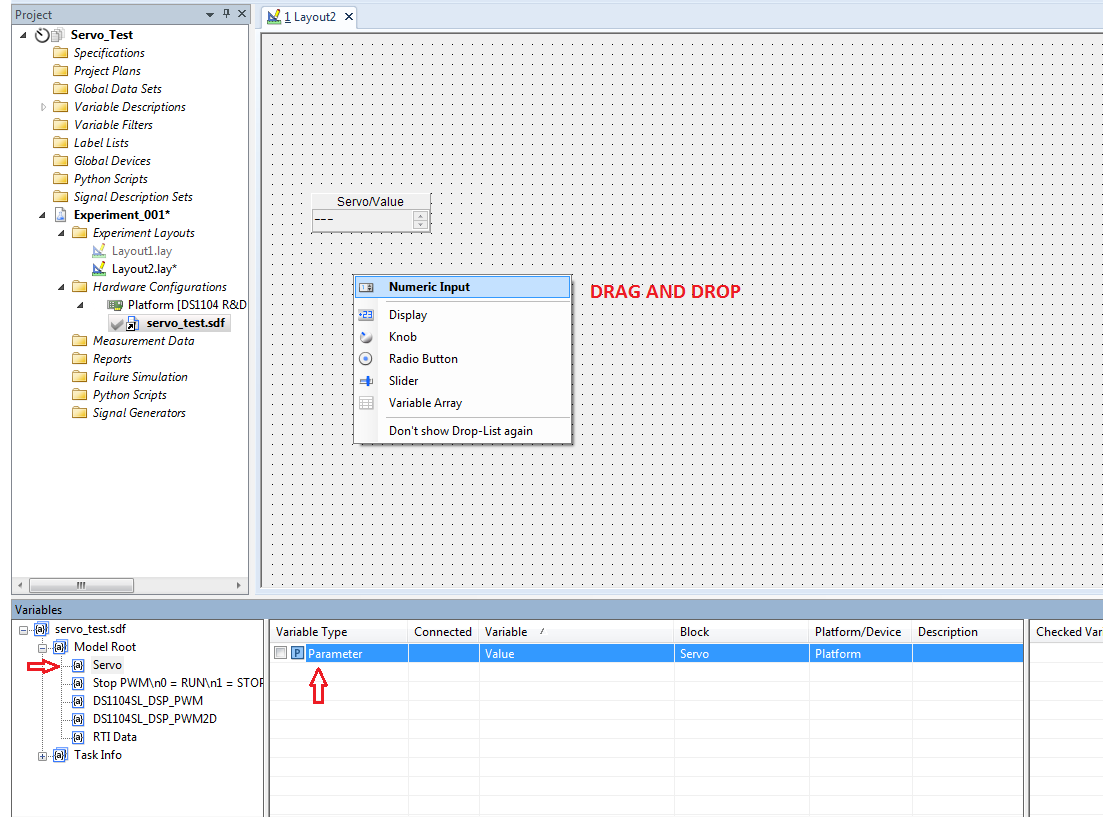
\includegraphics[width=0.8\textwidth]{Images/Ball and Bean/ControlDesk/CD10.png}
        \caption{Servo numeric input}
        \label{fig33}
    \end{figure}
    \begin{figure}[H]
        \centering
        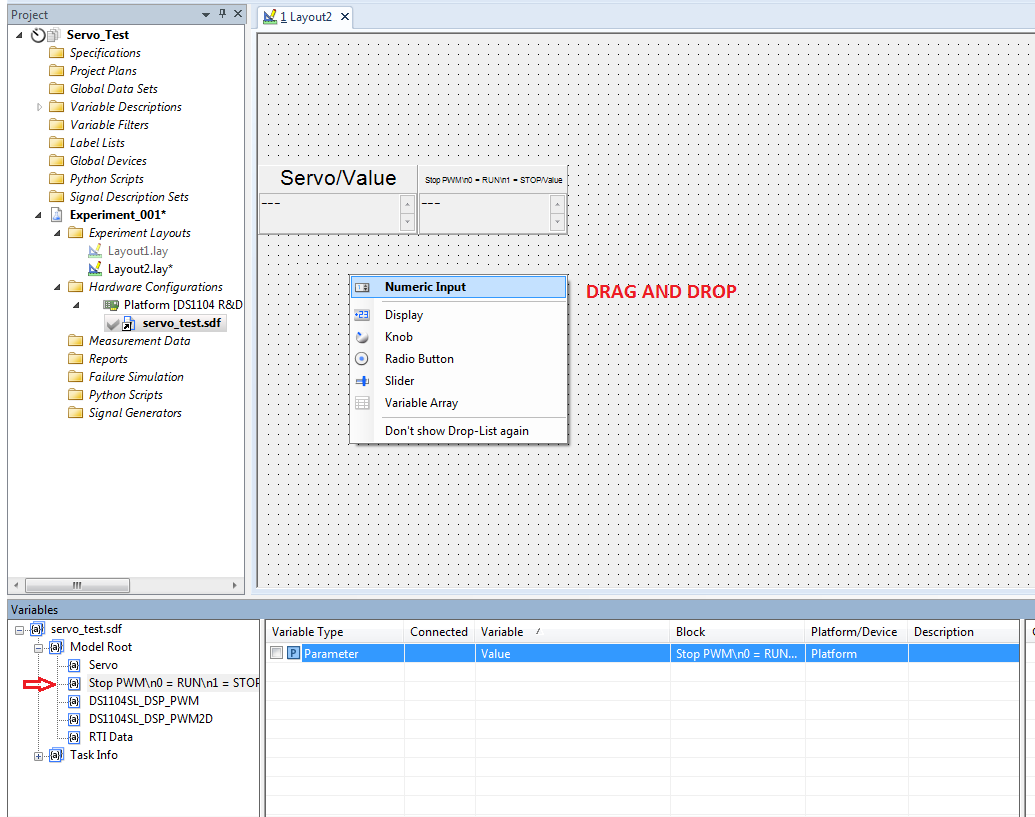
\includegraphics[width=0.8\textwidth]{Images/Ball and Bean/ControlDesk/CD11.png}
        \caption{START/STOP numeric input}
        \label{fig34}
    \end{figure}
    \begin{figure}[H]
        \centering
        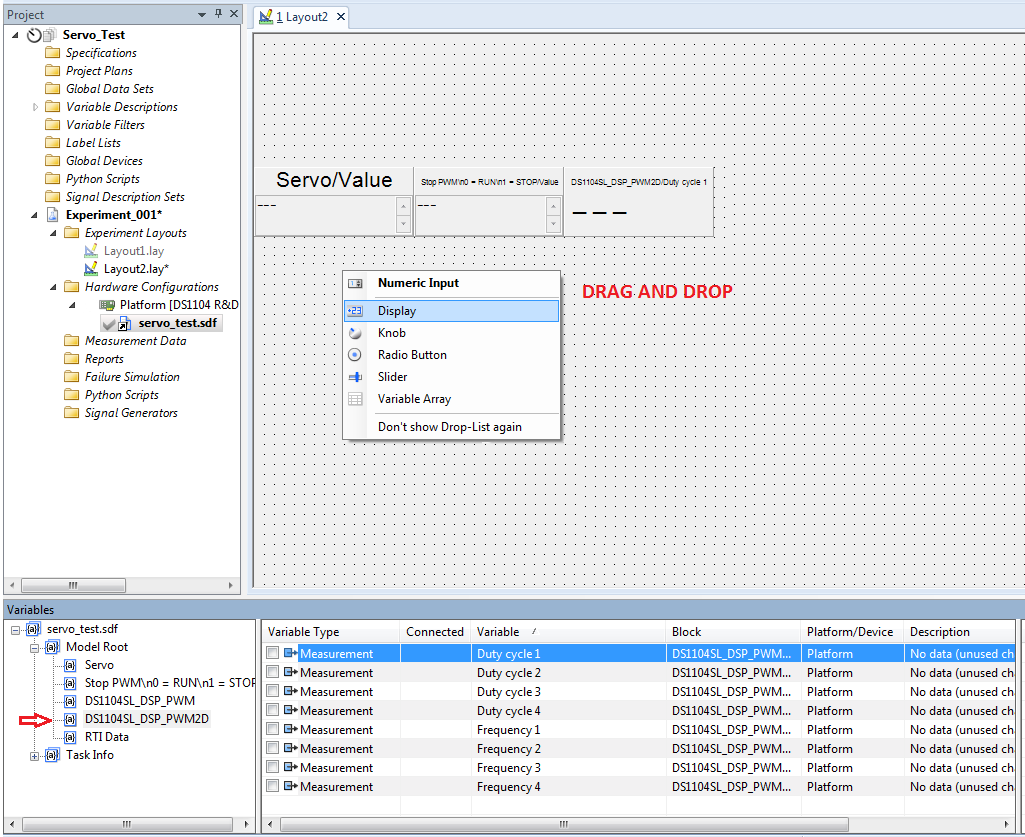
\includegraphics[width=0.8\textwidth]{Images/Ball and Bean/ControlDesk/CD12.png}
        \caption{PWM numeric display}
        \label{fig35}
    \end{figure}
    \begin{figure}[H]
        \centering
        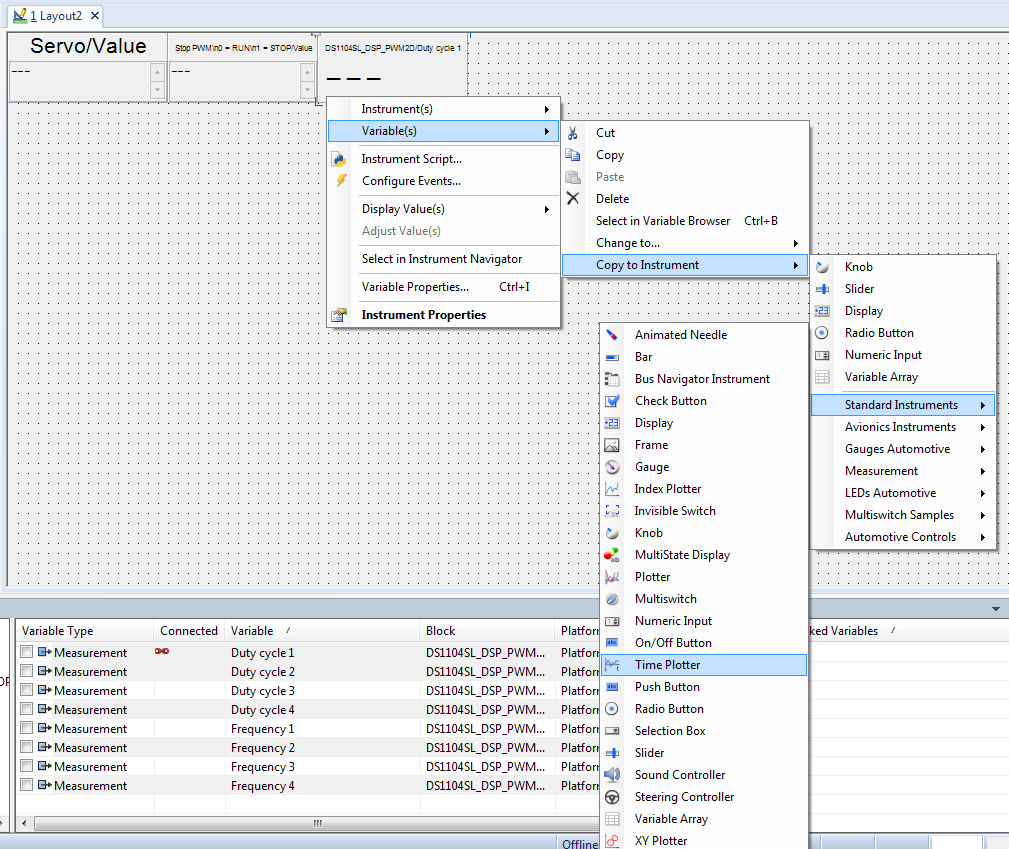
\includegraphics[width=0.8\textwidth]{Images/Ball and Bean/ControlDesk/CD13.png}
        \caption{Adding plotter linked to PWM duty cycle}
        \label{fig36}
    \end{figure}
With these items, you can now press the \textcolor{green}{\textbf{Go Online}} and \textcolor{blue}{\textbf{Start Measuring}} buttons to test the experiment.

\newpage

\section{Ball and beam hardware and Simulink modeling}
The objective of this project is the practical implementation of a ball and beam system using the dSPACE digital control system. The main components are a servomotor, as actuator, were the beam is attached, and an ultrasonic sensor HC-SR04, as an element to measure error. \par
The \textbf{DS1104 Slave DSP F240 blocks}, above mentioned, were used to do the control tasks of the ball and beam system.\par
\subsection{About the hardware}
For the main structure, a didactic robot with five degrees of freedom was used, where the base arm was fixed to avoid involuntary movements.\par
The HC-SR04 ultrasonic sensor was placed at one end of the beam together with the beam servo.\par
The beam has parallel lines where the ball is supported. This ball has a diameter of 8 cm, which is sufficient for the sensor to detect it at the end of the beam.\par
For the electrical connections, a PCB was designed using the free software for electronic design, \textbf{KiCAD}. The electrical characteristics concerning supply voltage and current consumption were extracted from the data sheets of the components. The servomotors have an independent power supply from the ultrasonic sensor. All components share GND in order to have a single reference.\par
The corresponding data sheets are attached at the end of the document.
    \begin{figure}[H]
        \centering
        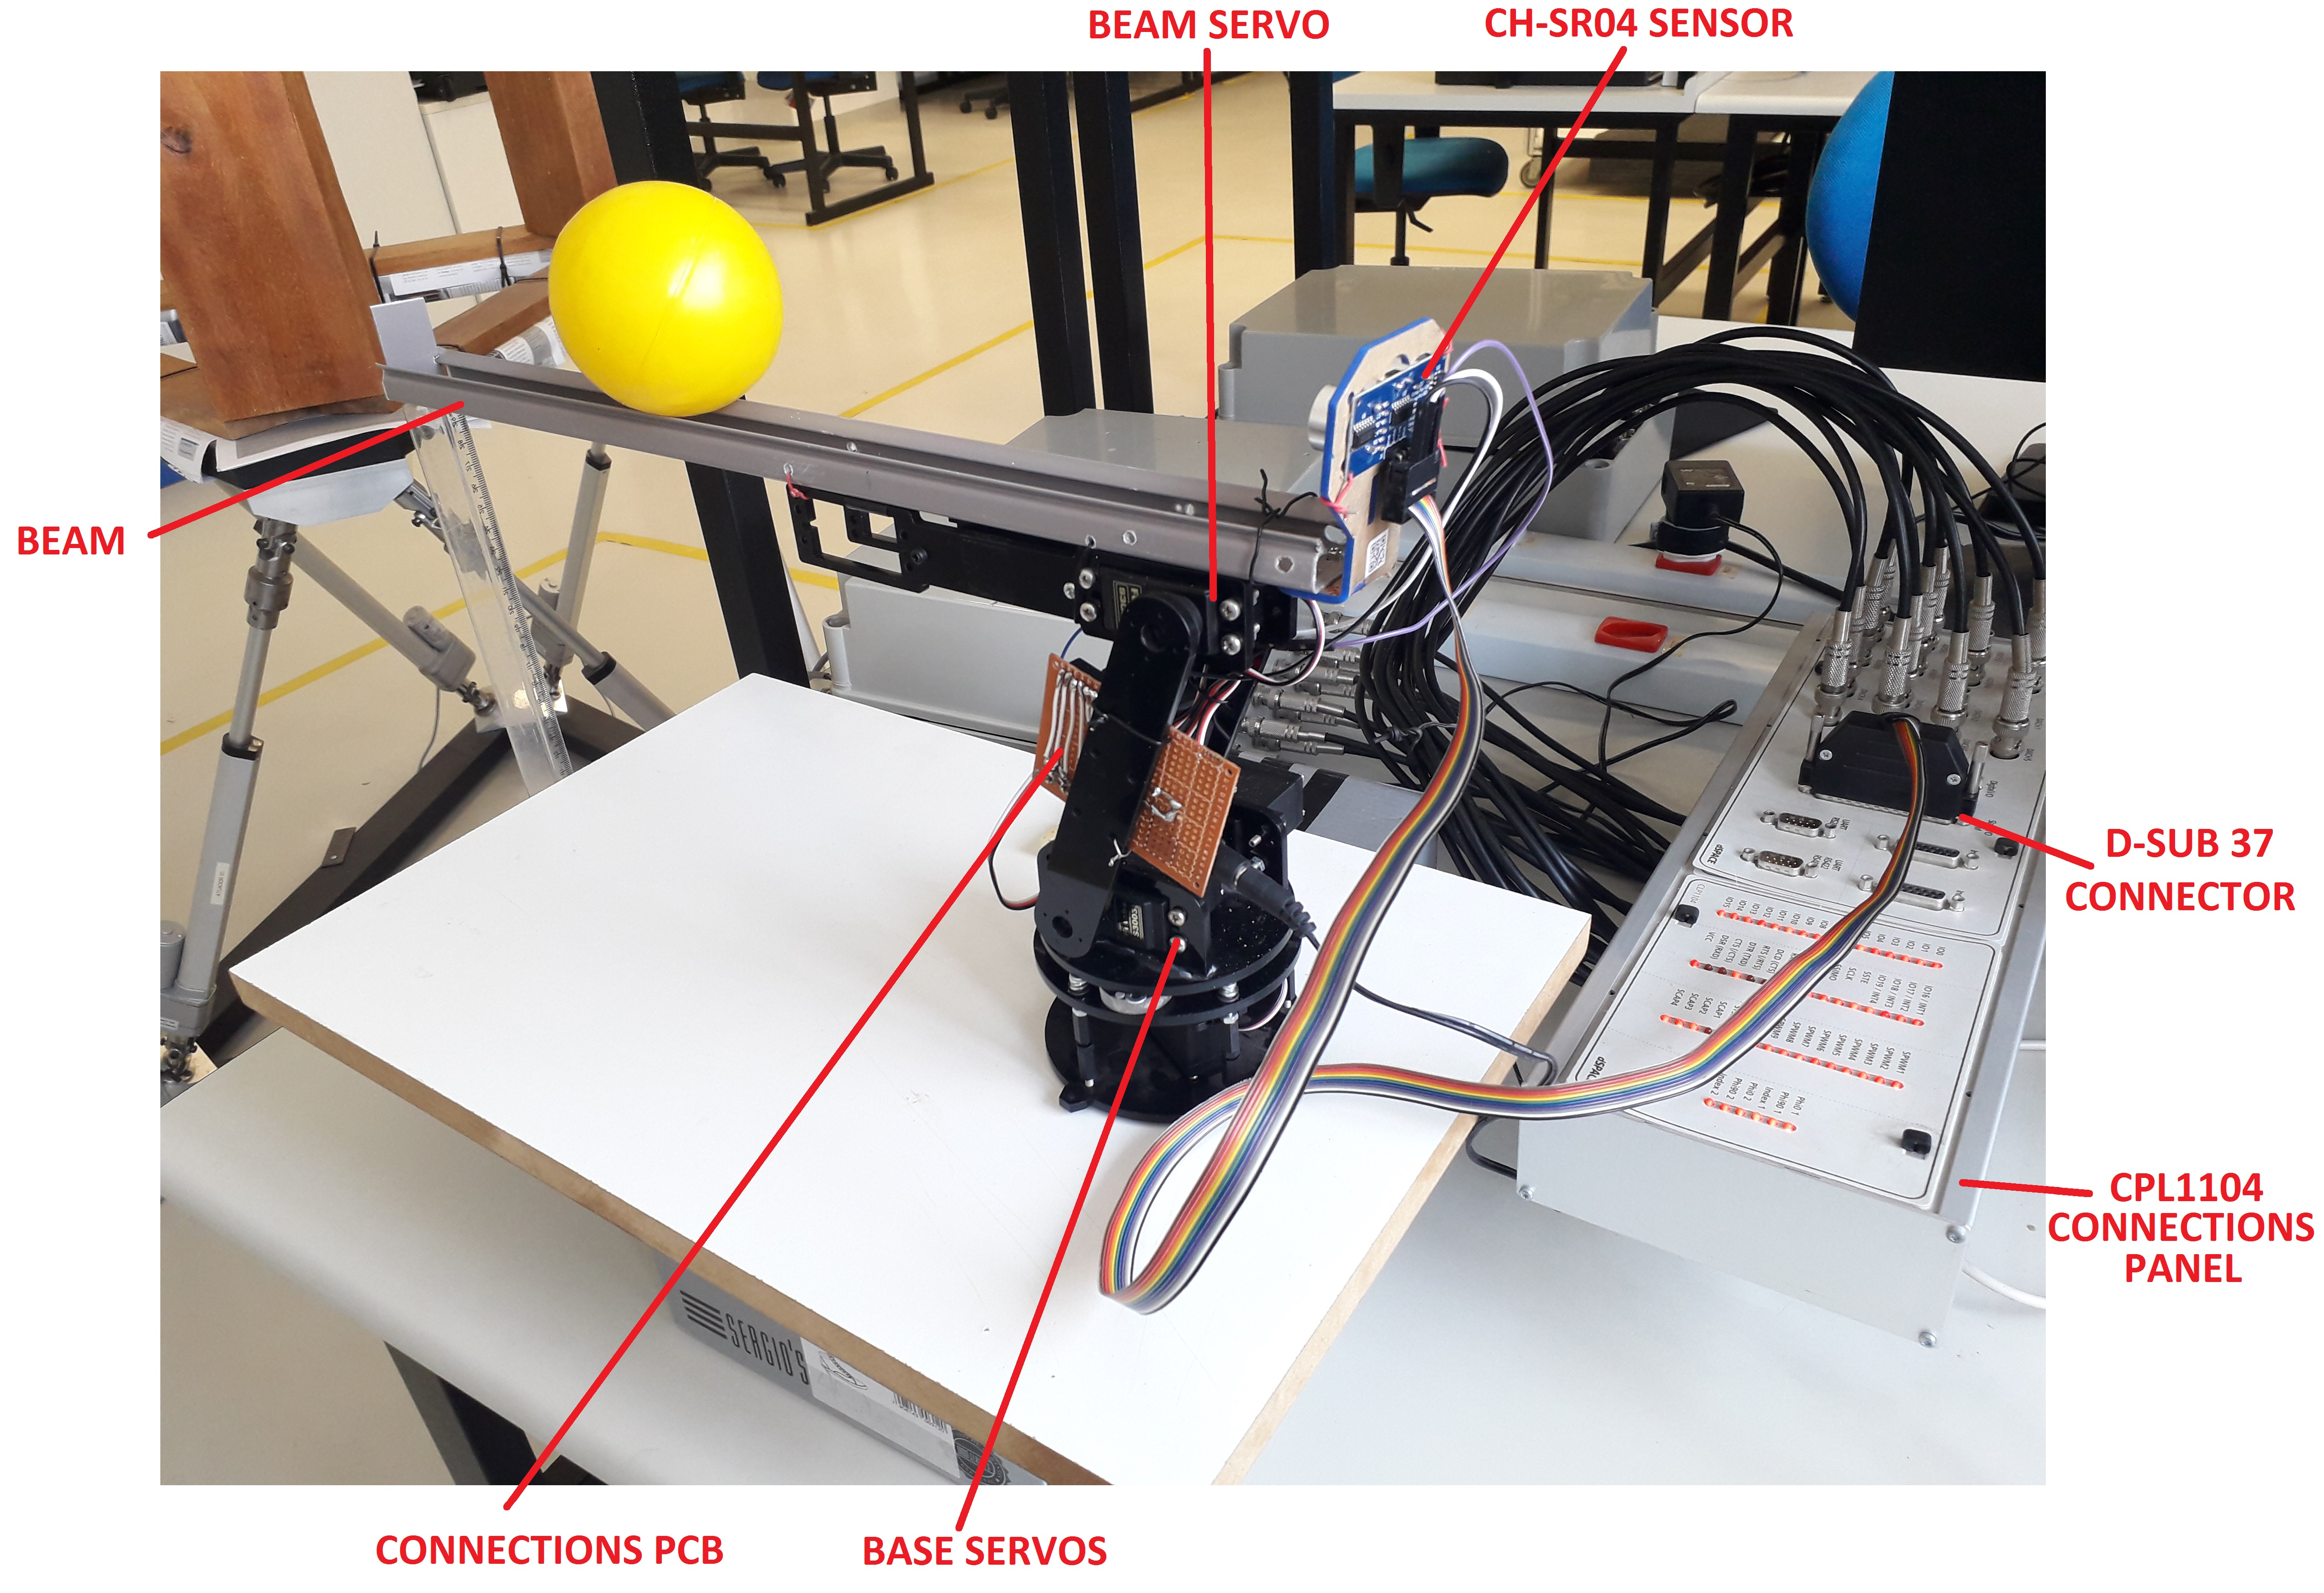
\includegraphics[width=\textwidth]{Images/Ball and Bean/Hardware/Parts.jpg}
        \caption{Ball and beam implementation using dSPACE digital control system}
        \label{fig41}
    \end{figure}
    
\subsection{Connection panel - KiCAD}
The connection panel was designed with the actual system in mind where there are two servomotors on the base, another on the beam and an ultrasonic sensor.
The power supply of the servomotors is independent of the sensor even though they have the same GND. The voltage for the servomotors is 6V.\par
Regarding control signals, in the schematic diagram it can be seen that the servomotors of the base are commanded with the same signal \textbf{SPWM8} and the servomotor of the beam with \textbf{SPWM7}. These are PWM signals where \textbf{SPWM8} has a constant value of 0.0775 equivalent to a pulse width of \textcolor{green}{\textit{1.55 ms}}.\par
The ultrasonic sensor HC-SR04 needs a minimum trigger pulse of 10 $\mu$s. For this, the \textbf{ST2PWM} signal is used, which sends the trigger pulse every 20ms. For the echo reading, the signal input \textbf{SCAP1} was used.\par
Inside the schematic a label indicating the current connection was left, which will have to be replaced once the connections PCB is available.
    \begin{figure}[H]
        \centering
        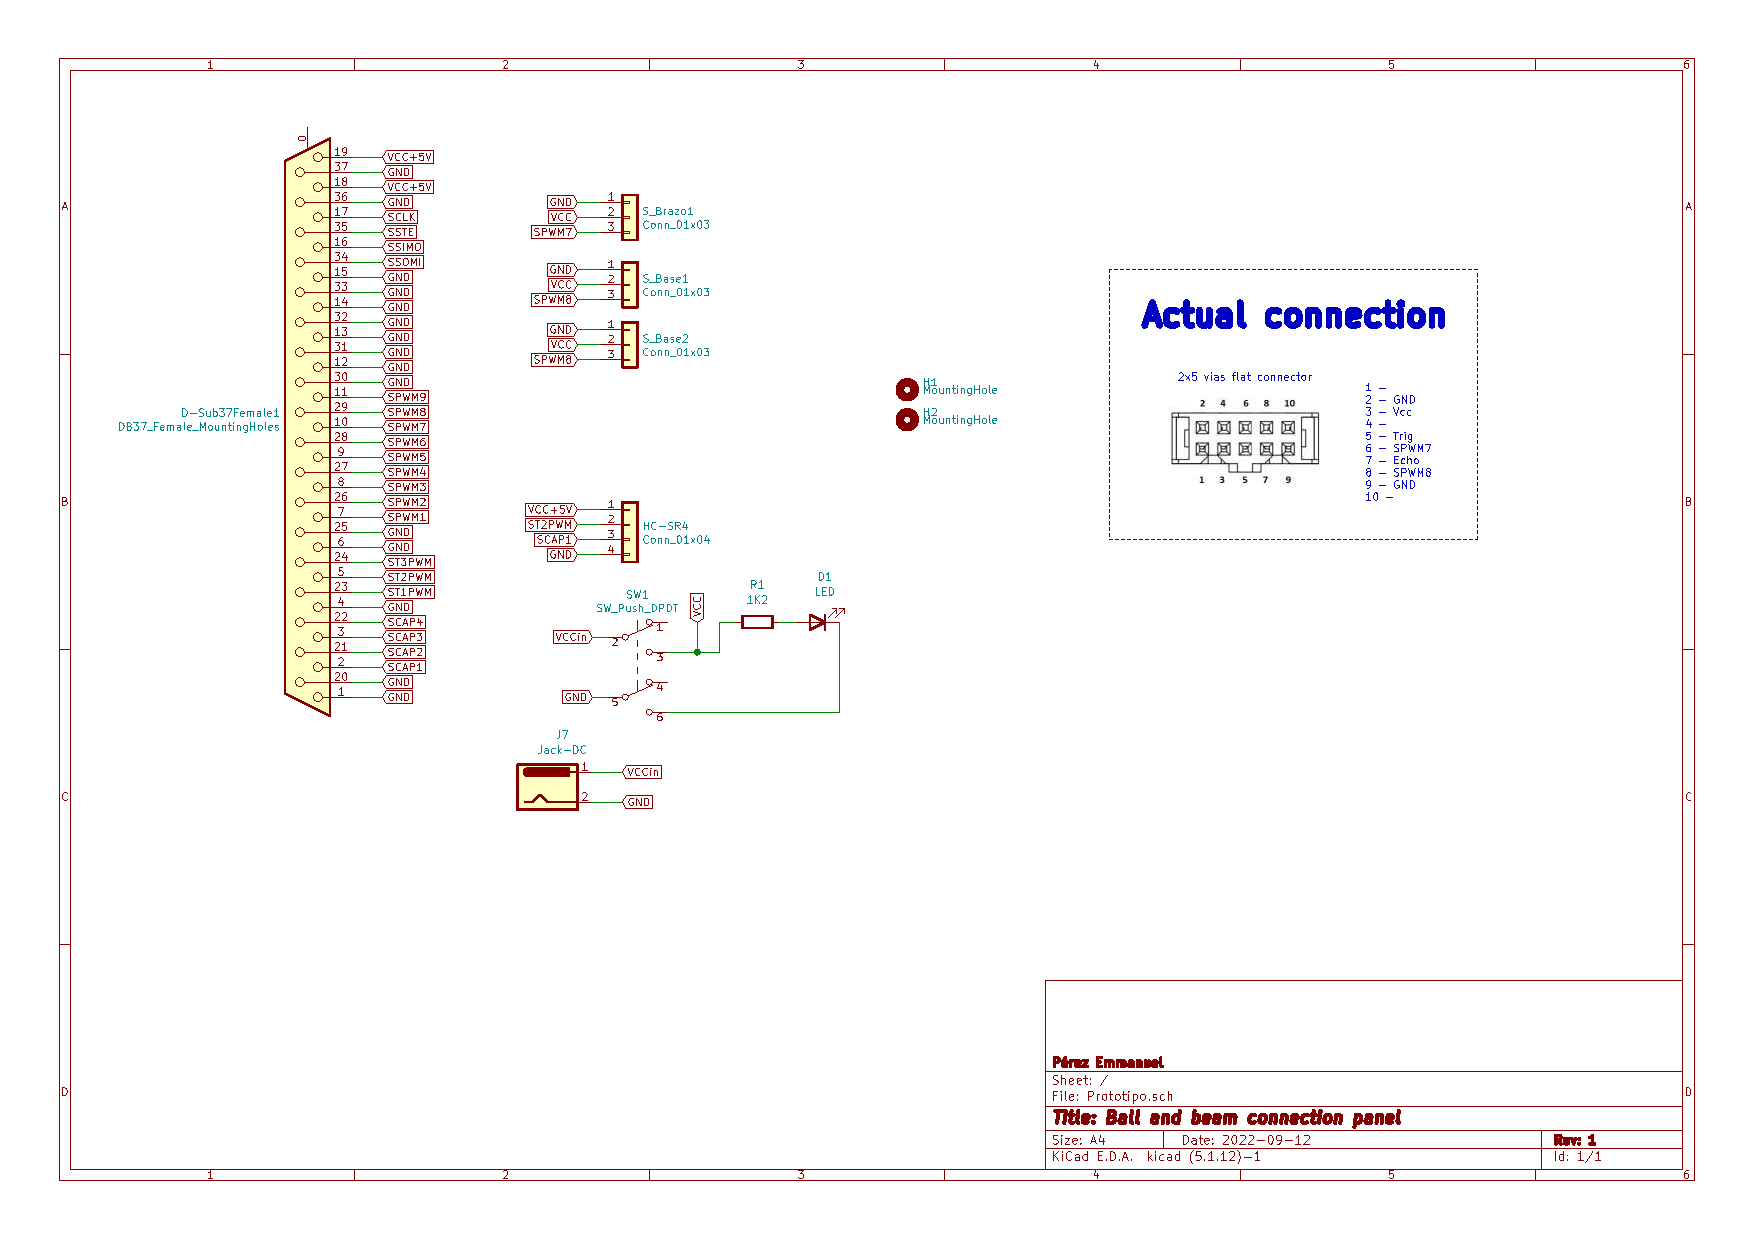
\includegraphics[width=\textwidth]{Images/Ball and Bean/Hardware/Ball and beam connection panel.pdf}
        \caption{Schematic diagram}
        \label{fig42}
    \end{figure}

    \begin{figure}[H]
        \centering
        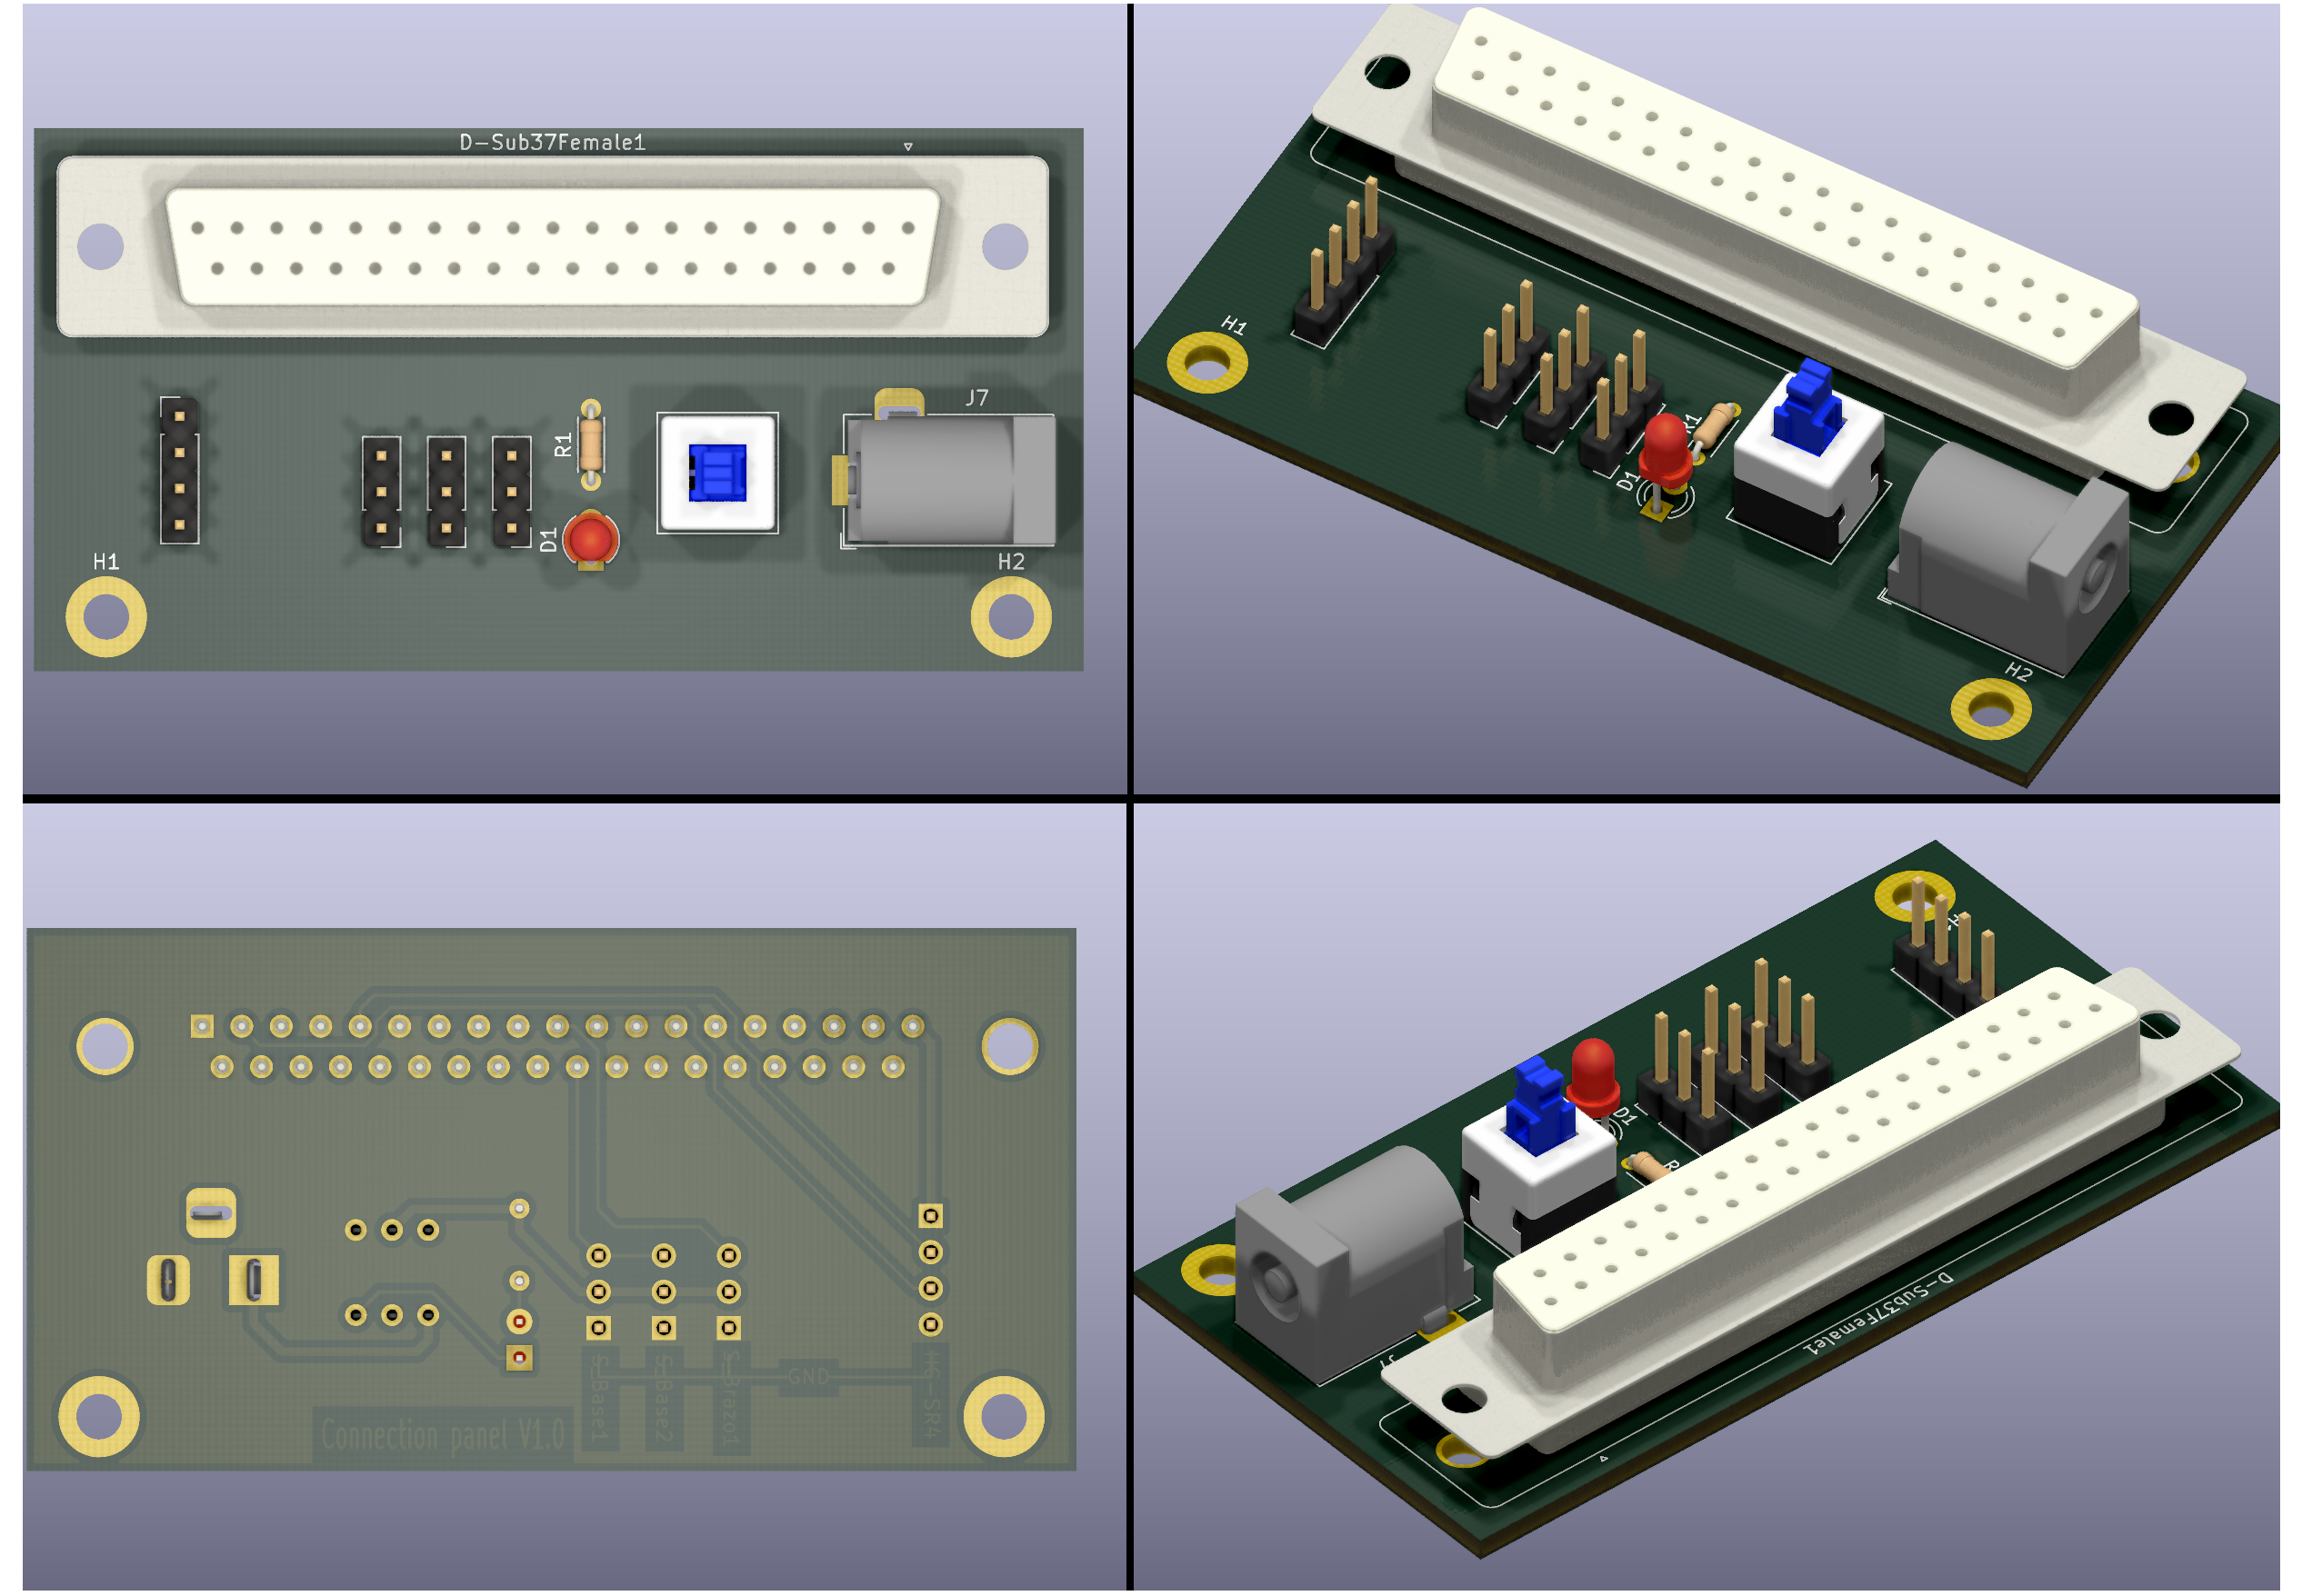
\includegraphics[width=\textwidth]{Images/Ball and Bean/Hardware/PCB.png}
        \caption{Final PCB}
        \label{fig43}
    \end{figure}

\subsection{Simulink model}
The control model that was designed is based on two main blocks of the DS1104 Slave DSP F240 Blockset library.
\begin{itemize}
    \item \textbf{DS1104SL\_DSP\_PWM}: used to generate the PWM and trigger signals.
    \item \textbf{DS1104SL\_DSP\_PWM2D}: used to read the echo from the ultrasonic sensor.
\end{itemize}
The plant controller was determined empirically. It would be necessary to apply control theory to determine all the characteristic values that define this system.
\begin{figure}[H]
    \centering
    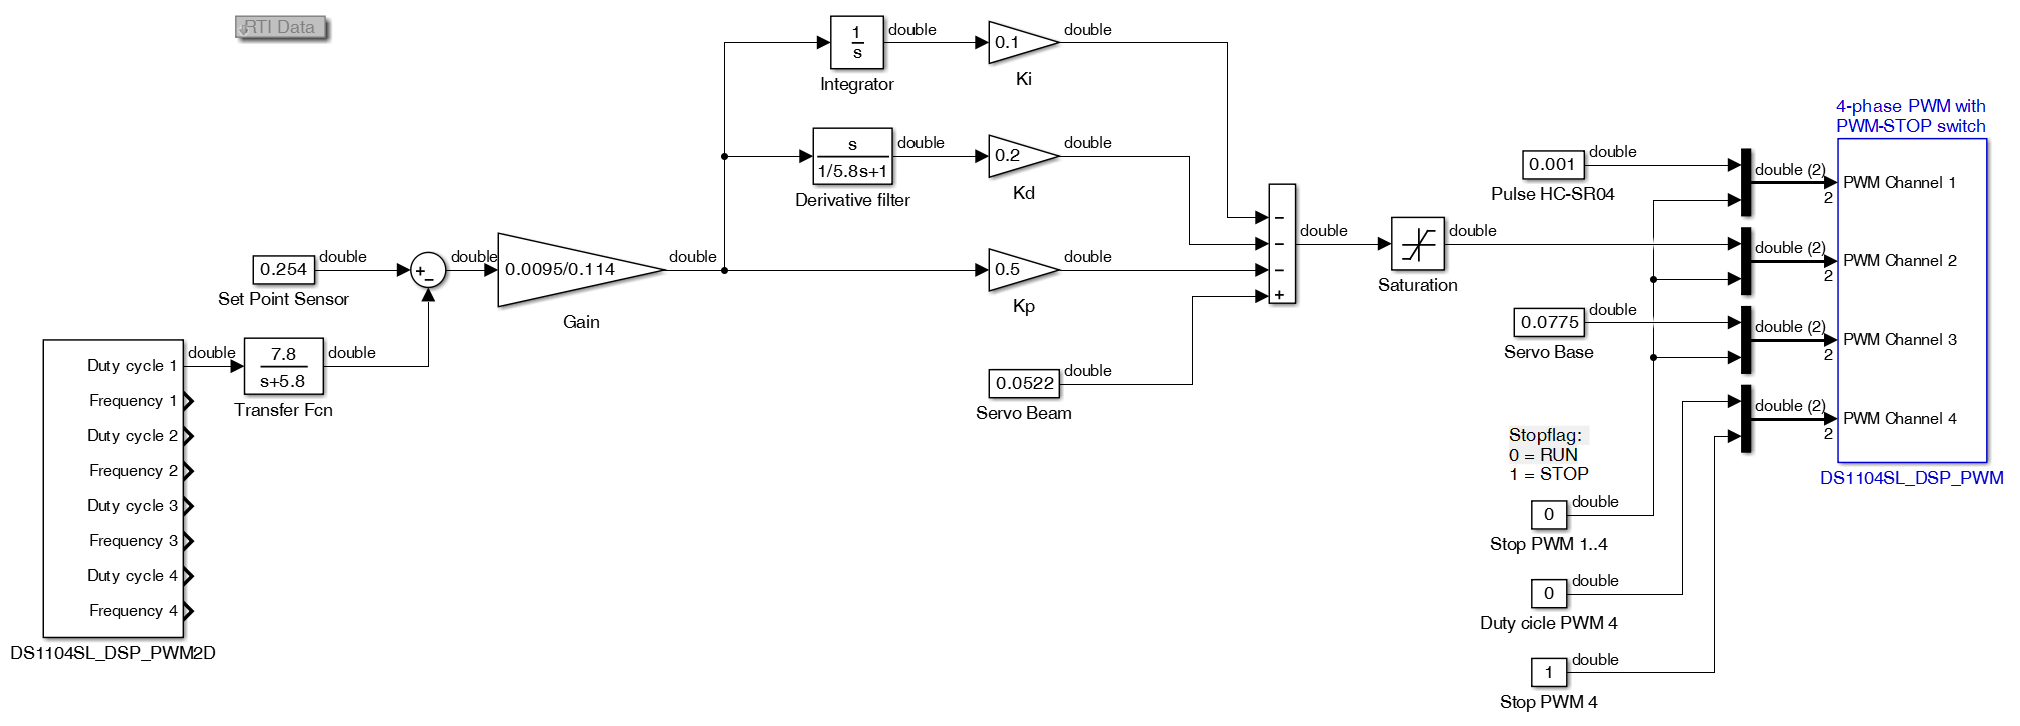
\includegraphics[width=\textwidth]{Images/Ball and Bean/Similink/Simulink-Controller.png}
    \caption{Simulink model}
    \label{fig46}
\end{figure}
\subsubsection{PWM generation}
For the generation of the PWM signals needed for this project, 3 inputs of the \textcolor{red}{\textbf{DS1104SL\_DSP\_PWM}} block were used. The block was programmed in asymmetric mode with a periodic pulse of 20 ms. Each channel has a MUX block where the START/STOP signal can be entered.
\begin{enumerate}
    \item \textbf{PWM Channel 1 - ST2PWM signal}: Used to set the pulse width of the trigger signal of the HC-SR04 ultrasonic sensor. A constant block with a value of \textbf{0.001} can be seen in the model. Multiplying this value by the period of the block gives the pulse width generated on channel 1 equal to 20 $\mu$s. 
    \begin{equation}
        Pulse_{Ch1} = 0,001 * 20 ms = 20 \mu s
    \end{equation}
    \item \textbf{PWM Channel 2 - SPWM7 signal}: Used to control the beam servo. In non-operational mode, it receives a constant value of 0.0522 which gives it a parallel position referenced to the base system. This is the rest position, which is reached when the error is zero.
    \begin{equation}
        Pulse_{Ch2} = 0,0522* 20 ms = 1,044 ms
    \end{equation}
   In this channel, a saturation block is applied to limit the servo's range of motion to prevent the beam from colliding with the base to which the robot is attached.
   \item \textbf{PWM Channel 3 - SPWM8 signal}: Used for fixed positioning of the base servomotors. This position corresponds to a position such that the servomotor of the beam is parallel to the base when it is in a rest position.\par
   A constant block with a value of \textbf{0.0775} can be seen in the model. Multiplying this value by the period of the block gives the pulse width generated on channel 3 equal to 1,55 ms. 
    \begin{equation}
        Pulse_{Ch3} = 0,0775* 20 ms = 1,55 ms
    \end{equation}
   \item \textbf{PWM Channel 4}: Disabled.
\end{enumerate}

\subsubsection{Echo pulse capture}
As our sensor returns a variable length pulse depending on the distance from the measurement object, the \textcolor{red}{\textbf{DS1104SL\_DSP\_PWM2D}} block is used. This block has the main function of capturing PWM pulses.
The Duty cycle 1 input will be used because the others are not necessary.\par
As this block is read only, no configuration is needed for this task.\par
The measured signal is smoothed by a TansferFcn block. The values of this block were determined empirically since at the time this file was written, no mathematical model of the system was implemented.
\subsubsection{About the error}
To establish the error and its scale, measurements were made using the ultrasonic sensor to determine the MIN and MAX limit values of the beam. In the following figure, these values and the convention adopted for the error can be seen graphically.
\begin{figure}[H]
    \centering
    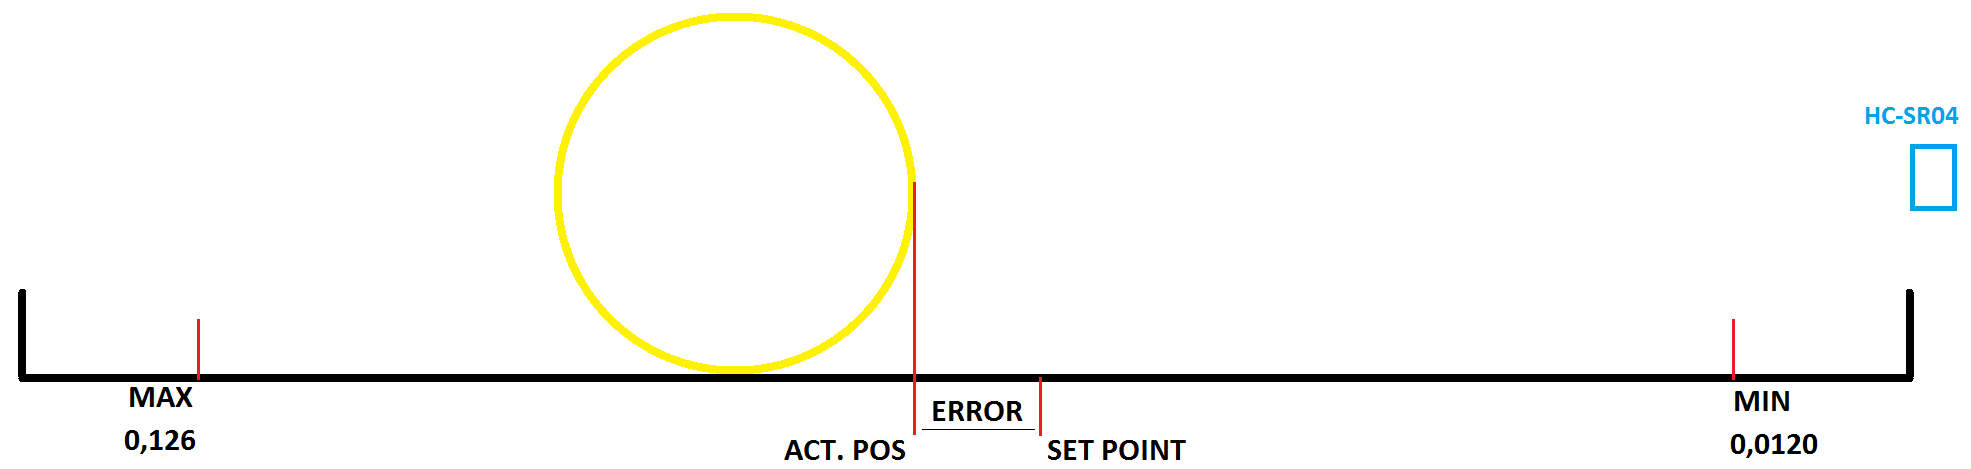
\includegraphics[width=\textwidth]{Images/Ball and Bean/Hardware/MAX-MIN.png}
    \caption{MAX and MIN values of the beam}
    \label{fig44}
\end{figure}
It is very important to note that these values change depending on how the trigger pulse is generated, i.e., its frequency, pulse width and mode (symmetric or asymmetric mode), and also on the geometry where the sound bounces. To exemplify the adopted convention, the data is taken from the figure \ref{fig44}.
    \noindent $SetPoint = 0,057$\\
    $ActPos = 0,092$\\
    $Error = SetPoint - ActPos = 0,057 - 0,092 = -0,035$\\
    So, we have a negative error value, but what does it mean?\par
As mentioned, limits were set for the range of motion of the beam servomotor. These limits correspond to $+0.0095$ and $-0.0095$ referred to the constant block of Channel 2 whose value is $0.0522$.
To see this in a graphical way the following figure is used:
\begin{figure}[H]
    \centering
    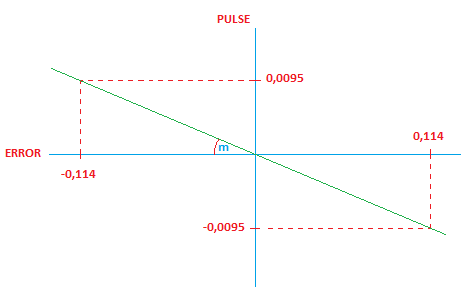
\includegraphics[width=\textwidth]{Images/Ball and Bean/Hardware/SCALE.png}
    \caption{PWM as a function of error }
    \label{fig45}
\end{figure}
In the model, the value of the slope m is entered as a gain block whose value:

\centering
\begin{math}
    m = \frac{0.0095}{0.114} = 0,0833    
\end{math}



